\documentclass{article}
\usepackage[utf8]{inputenc}

% Formatting
\usepackage[utf8]{inputenc}
\usepackage[margin=0.8in]{geometry}
\usepackage[titletoc,title]{appendix}
\usepackage{multicol}
\usepackage{enumitem}
\setlist[itemize]{leftmargin=4mm}

% Math
\usepackage{amsfonts,amssymb,mathtools}
\usepackage{centernot}

% Images
\usepackage{graphicx}
\graphicspath{{./images/}}

\title{CS1231S 2020 Cheatsheet}
% \author{}
\date{}

\begin{document}

%\maketitle

% ==================================================
\section*{Types of Proofs}
% ==================================================
\begin{multicols}{2}
\begin{itemize}
    \item Direct Proof
    \item Proof by Construction
    \item Disproof by Counter Example
    \item Proof by Exhaustion
    \item Proof by Deduction
    \item Proof by Contradiction
    \item Proof by Contraposition
    \item Proof by Mathematical Induction
    \item Combinatorial Proof
\end{itemize}
\end{multicols}

% ==================================================
\section*{Logical Form and Logical Equivalence}
% ==================================================
\begin{center}
    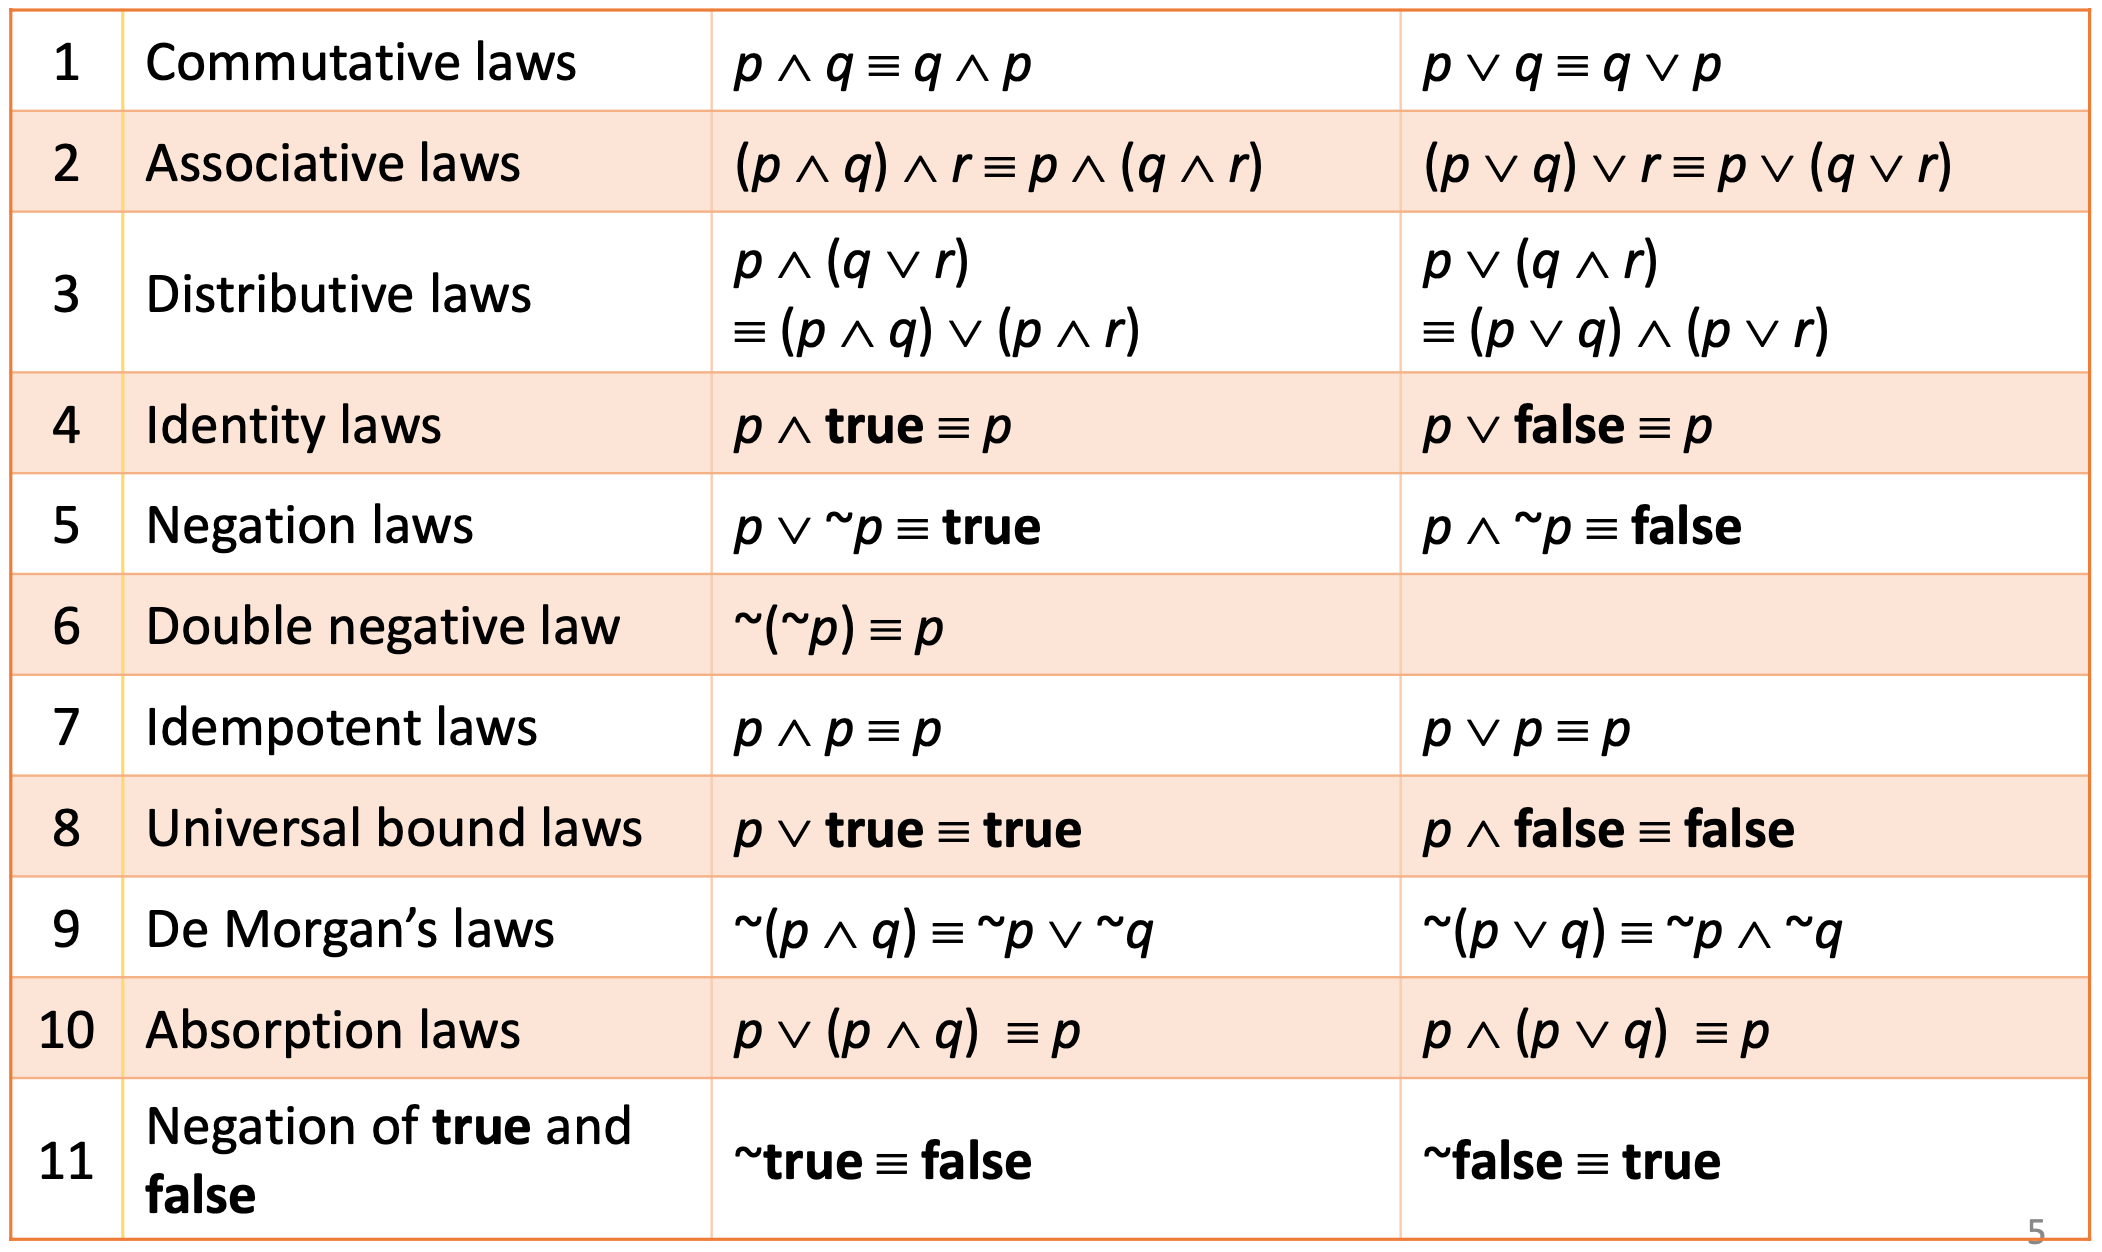
\includegraphics[width=12cm]{images/theorem2.1.1.png}
\end{center}

\begin{itemize}
    \item Conditional Statements and Implication Law: $p\xrightarrow{} q \equiv \ \sim p \vee q$
    \item Negation of Conditional: $\sim (p\xrightarrow{} q) \equiv \ p \  \land \sim q$
    \item Contrapositive: $\sim q \xrightarrow[]{} \ \sim p$
    \item Converse: $q \xrightarrow{} p$
    \item Inverse: $\sim p \xrightarrow{} \ \sim q$
    \item Biconditional $p \xleftrightarrow{} q \equiv (p \xrightarrow{} q) \wedge (q\xrightarrow{}p)$
\end{itemize}
\begin{center}
    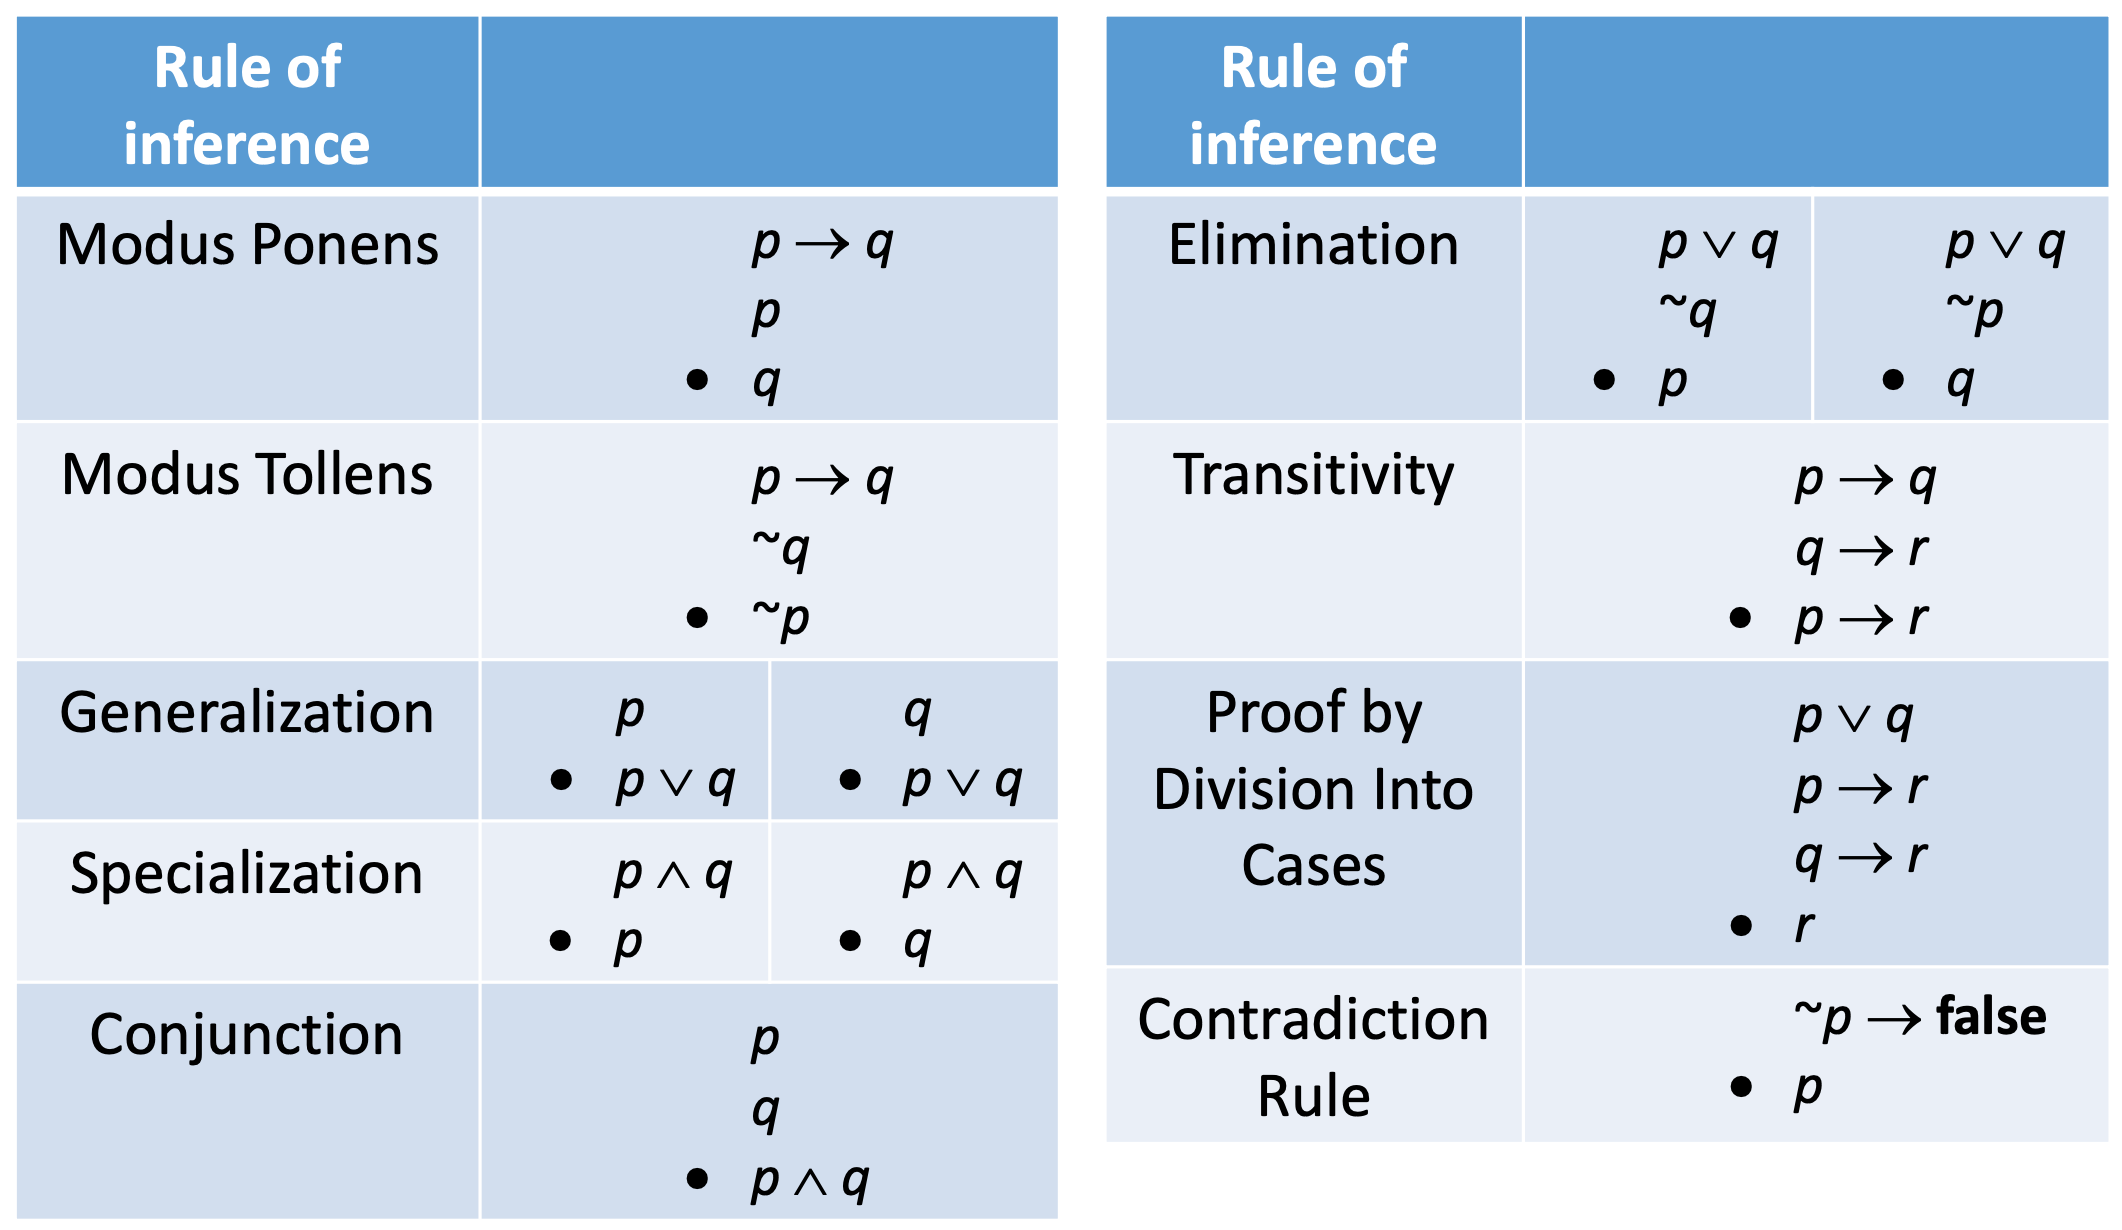
\includegraphics[width=12cm]{images/rulesofinference.png}
\begin{itemize}
    \item Tutorial 2 Q8a: $(\forall x \in D \ P(x))\land(\forall x \in D \ Q(x)) \xleftrightarrow{} \forall x \in D (P(x) \land Q(x))$
    \item Tutorial 2 Q8b: $(\exists x \in D \ P(x)) \land (\exists x \in D \ Q(x))$ and $\exists x \in D (P(x) \land Q(x))$ are NOT equivalent.
\end{itemize}
\end{center}

% ==================================================
\section*{Number Definitions and Theorems}
% ==================================================
\begin{multicols}{2}
    \begin{itemize}
        \item Even Numbers: $n=2k$ for some $k \in \mathbb{Z}$
        \item Odd Numbers: $n=2k+1$ for some $k \in\mathbb{Z}$
        \item Rational Numbers: $r=\frac{a}{b}$ and $b\neq0$
    \end{itemize}
\end{multicols}

\begin{itemize}
    \item Theorem 4.3.1: Every integer is a rational number.
    \item Theorem 4.3.2: The sum of any two rational numbers is rational.
    \item Corollary 4.2.3: The double of a rational number is rational.
    \item Theorem 4.6.1: There is no greatest integer.
    \item Proposition 4.7.4: For all integers $n$, if $n^2$ is even, then $n$ is even.
    \item Theorem 4.8.1: $\sqrt{2}$ is irrational.
    \item Corollary 8.1.21: Let $n\in \mathbb{Z}$. Then $n$ is either even or odd, but not both.
    \item Tutorial 1 Q9: The product of any 2 odd integers is an odd integer
    \item Tutorial 1 Q10: If $a,b,c$ are integers such that $a^{2} + b^{2} = c^{2}$, then $a,b$ cannot both be odd.
    \item Tutorial 2 Q3: $\forall a,b,c \in \mathbb{Z}$, if $a - b$ is even and $a - c$ is even, then $b - c$ is even
    \item Assignment 1 Q7: Let $a$ be a rational number and $b$ an irrational number. Then $a \neq 0 \xrightarrow{} ab is irrational$.
    \item Assignment 1 Q8: $\forall n \in \mathbb{Z}, n^2 + n$ is even.
\end{itemize}

% ==================================================
\section*{Sets}
% ==================================================
\begin{itemize}
    \item Definition 5.1.3: Roster Notation (listing out all elements of the set) $\{1,2,3\}$
    \item Definition 5.1.5: Set-Builder Notation $\{x\in U: P(x)\}$
    \item Definition 5.1.9: Two sets are equal if and only if they have the same elements.
    \item Definition 5.1.15: The set with no element is called the empty est. It is denoted by $\varnothing$.
    \item Definition 5.2.1: The set of all subsets of A, denoted $P(A)$, is called the power set of A.
    \item Theorem 5.2.4: Suppose A is a finite set. Then $|P(A)| = 2^{|A|}$.
    \item Definition 5.2.6: An ordered pair is an expression of the form $(x,y)$. Let $(x,y)$ and $(x',y')$ be ordered pairs. Then $(x,y)=(x',y')$ if and only if $x=x'$ and $y=y'$.
    \item Definition 5.2.8: Let A, B be sets. The Cartesian product of A and B, denoted A $\times$ B, is defined to be $\{(x,y):x\in A$ and $y\in B\}$
    \item Theorem 5.3.11: Let A, B be disjoint finite sets. Then $|A\cup B|=|A|+|B|$. 
       \\ Let $A_1, A_2,...,A_n$ be pairwise disjoint finite sets. Then $|A_1|+|A_2|+...+|A_n|$.

    \begin{center}
        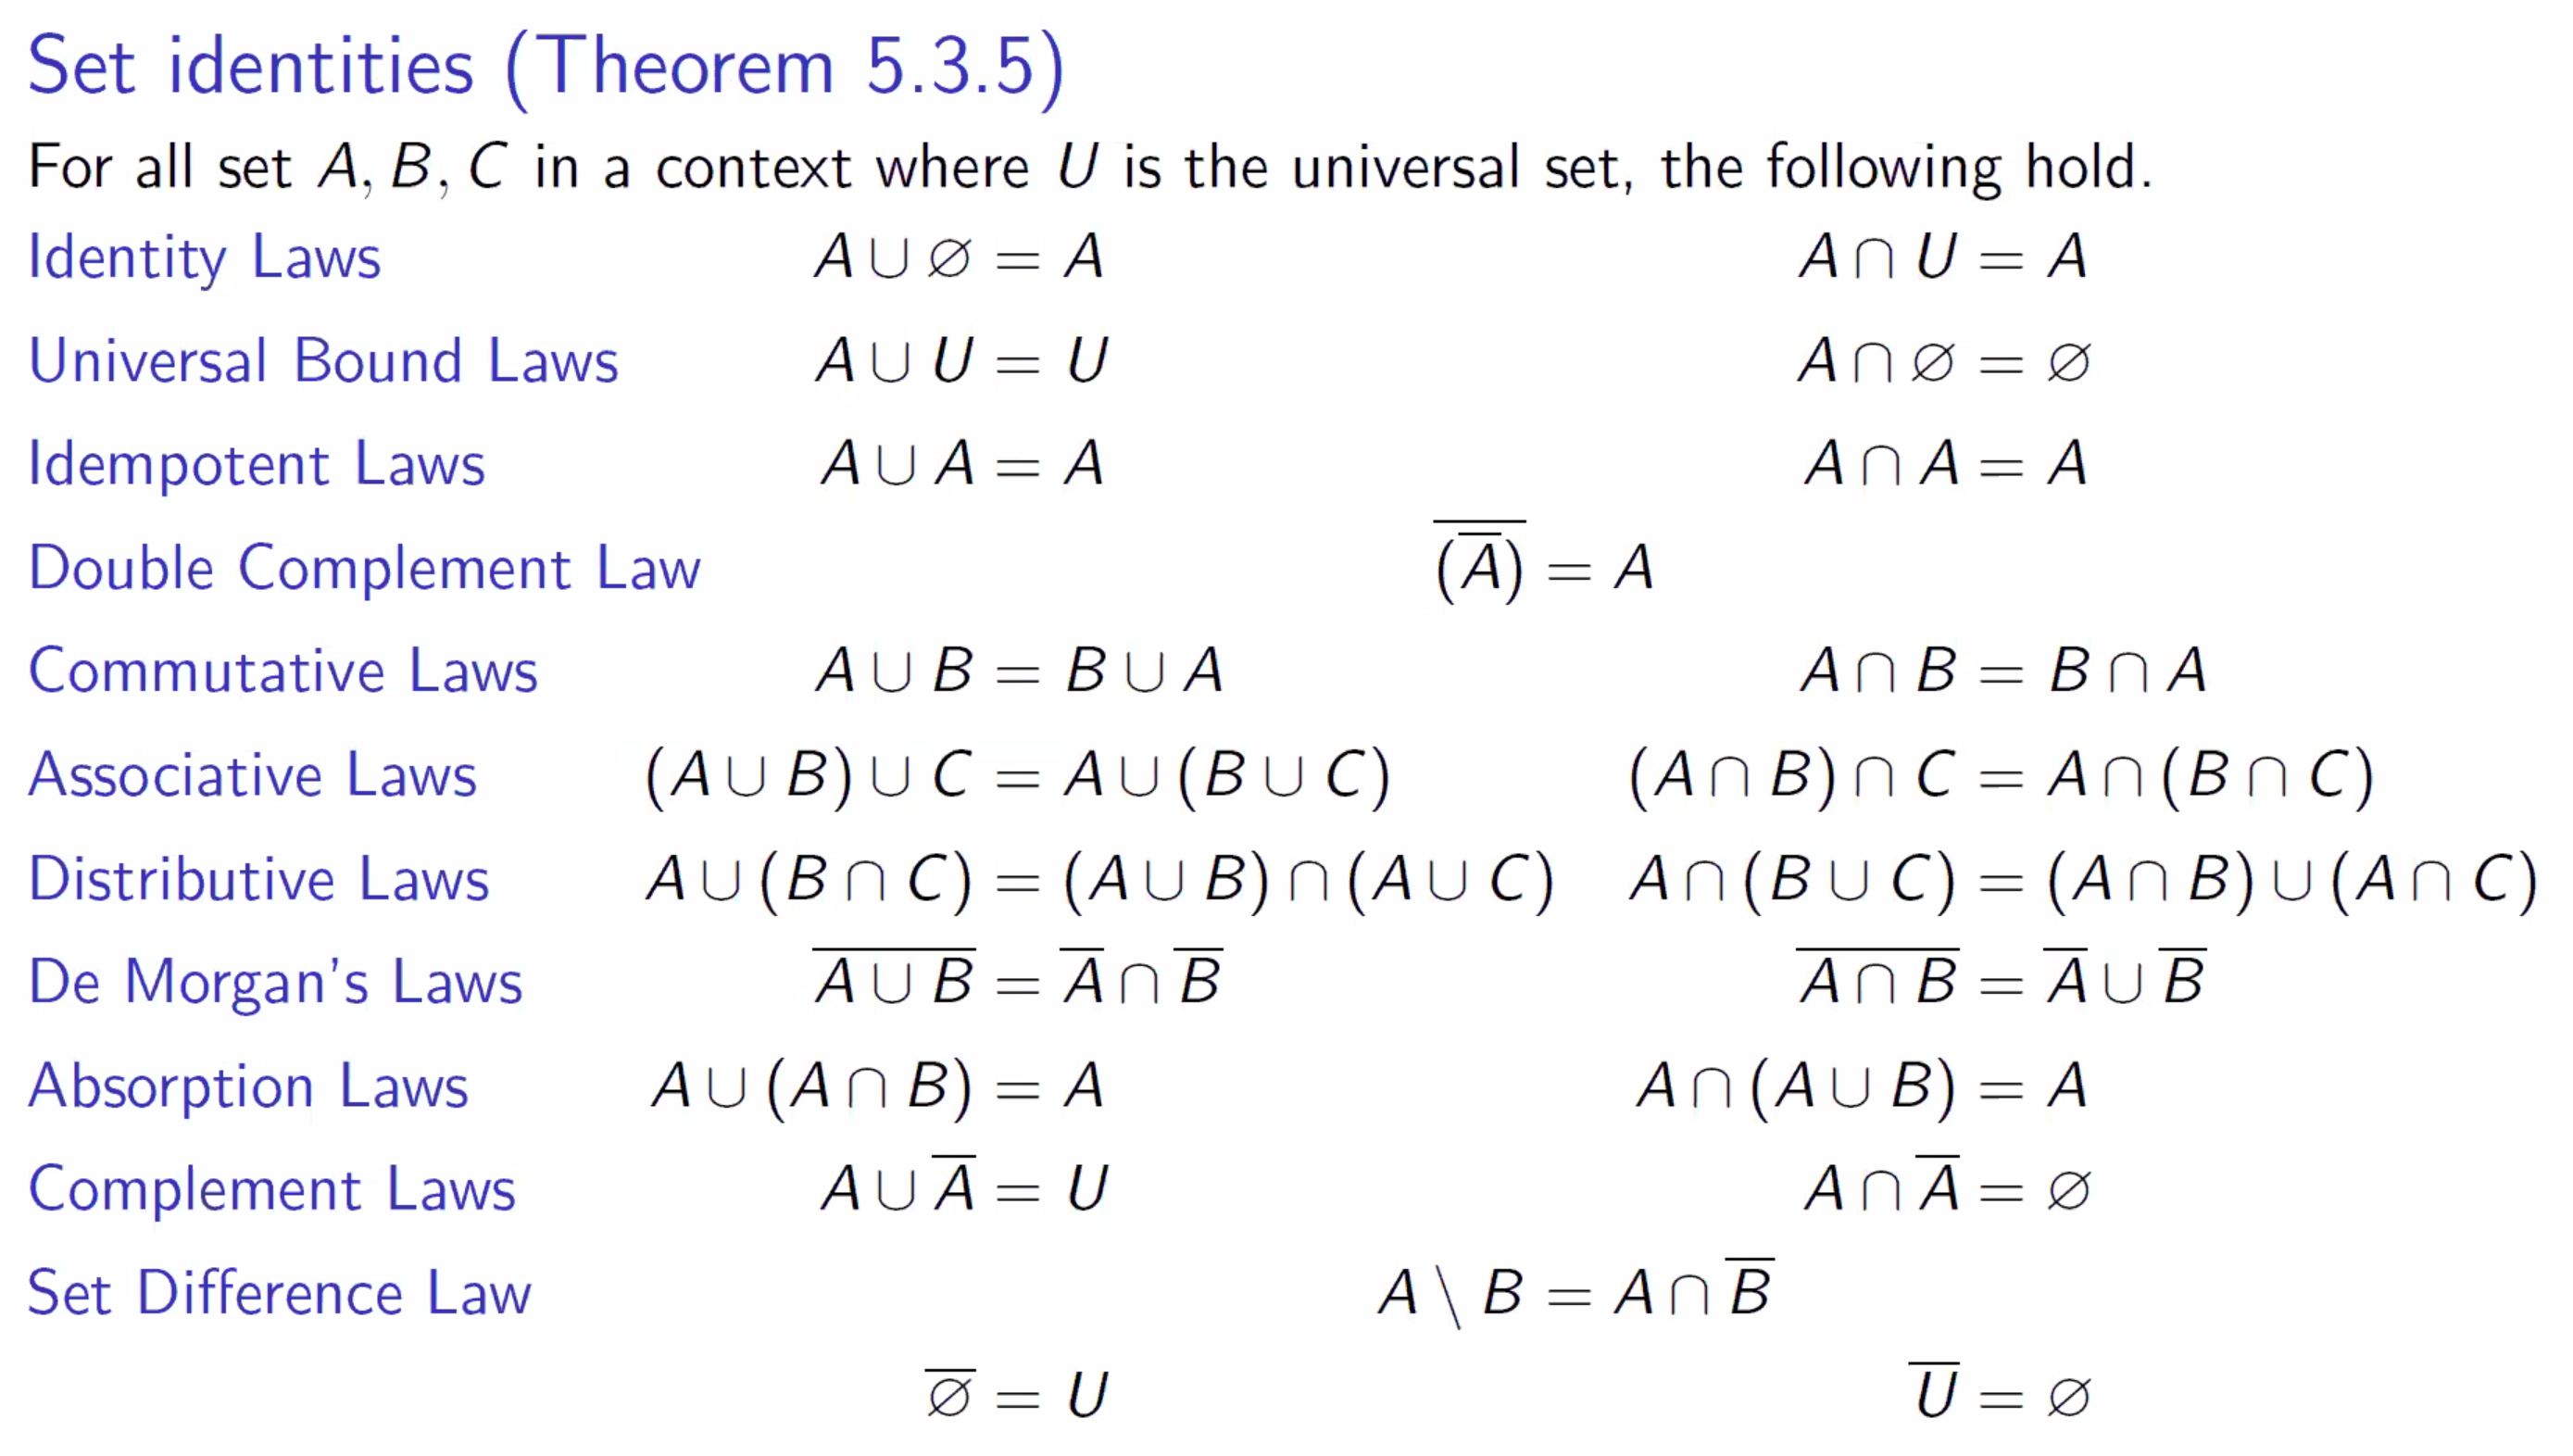
\includegraphics[width=12cm]{images/setidentities.png}
    \end{center}

    \item Tutorial 3 Q4: Let A = \{2n + 1 : $n \in \mathbb{Z}$\} and B = \{2n - 1 : $n \in \mathbb{Z}$\}. Then A = B.
    \item Tutorial 3 Q7: $A \cap (B \backslash C)=(A \cap B) \backslash C$
    \item Tutorial 3 Q8: $(A \cup \overline{B}) \cap (\overline{A} \cup B) = (A \cap B) \cup (\overline{A} \cap \overline{B})$
    \item Tutorial 3 Q9: $A \subseteq B \xleftrightarrow{} A \cup B = B$
    \item Assignment 1 Q11a: If $P(A \cup B) \subseteq P(A) \cup P(B)$, then either $A \subseteq B$ or $B \subseteq A$.
\end{itemize}

% ==================================================
\section*{Functions}
% ==================================================
\begin{itemize}
    \item Definition 6.1.1 (Function): A function or a map from A to B is an assignment to each element of A exactly one element of B. We write $f: A \xrightarrow{} B$ for "f is a function from A to B"
    \item Terminology 6.1.18 (Well Definition): A function is well-defined if its definition ensures that every element of the domain is assigned exactly one element of the codomain
    \item Definition 6.1.19 (Equality of Functions): Two functions $f: A \xrightarrow{} B$ and $g: C \xrightarrow{} D$ are equal if:
        \begin{center}
            (1) $A = C$ and $B = D$; and 
            \\ (2) $f(x) = g(x)$ for all $x \in A$
        \end{center}
    \item Definition 6.1.22 (Function Composition): Let $f: A \xrightarrow{} B$ and $g: \xrightarrow{} C$. Then $g \circ f: A \xrightarrow{} C$ such that for every $x \in A$, $(g \circ f)(x) = g(f(x))$
    \item Functions Compositions are non-commutative, but associative
    \item Definition 6.2.1 (Setwise image and preimage):
        \\ Let $f: A \xrightarrow{} B$.
        \\ \hspace*{3mm} (1) If $X \subseteq A$, then let $f(X) = \{y \in B: y = f(x)$ for some $x \in X\} = \{f(x): x \in X\}$
        \\ \hspace*{3mm} (2) If $Y \subseteq B$, then let $f^{-1}(Y) = \{x \in A: y=f(x)$ for some $y \in Y\}$
        \\ We call $f(X)$ the image of X, and $f^{-1}(Y)$ the preimage of $Y$ under $f$
    \item Definition 6.2.5 (Surjection, Injection, Bijection):
        \\ \hspace*{3mm} (1) $f$ is \emph{surjective} if $\forall y \in B \ \exists x \in A \ (y = f(x))$
        \\ \hspace*{3mm} (2) f is \emph{injective} if $\forall x,x' \in A \ (f(x) = f(x') \xrightarrow{} x = x')$
        \\ \hspace*{3mm} (3) f is \emph{bijective} if it is surjective and injective, i.e., $\forall y \in B \ \exists! x \in A \ (y=f(x))$ 
        \bigskip
    \item Prove Surjectivity:
        \\ Example 6.2.6: The function $f: \mathbb{Q} \xrightarrow{} \mathbb{Q}$, defined by setting $f(x)=3x+1$ for all $x \in \mathbb{Q}$, is surjective.
        \bigskip
        \\ Proof:
        \\ \hspace*{3mm} 1. Take any $y \in \mathbb{Q}$.
        \\ \hspace*{3mm} 2. Let $x=(y-1)/3$.
        \\ \hspace*{3mm} 3. Then $x \in \mathbb{Q}$ and $f(x) = 3x+1=y$.
    \item Prove Non-surjectivity:
        \\ - Remark 6.2.7(2): A function $f:A\xrightarrow{} B$ is not surjective if and only if $\exists y \in B \ \forall x \in A\ (y\neq f(x))$
        \bigskip
        \\ Example 6.2.8: Define $g: \mathbb{Z} \xrightarrow{} \mathbb{Z}$ by setting $g(x) = x^2$ for every $x \in \mathbb{Z}$. Then $g$ is not \mbox{surjective}.
        \bigskip
        \\ Proof:
        \\ \hspace*{3mm} 1. Note $g(x) = x^2 \geq 0 > -1$ for all $x \in \mathbb{Z}$.
        \\ \hspace*{3mm} 2. So $g(x) \neq -1$ for all $x \in \mathbb{Z}$, although $-1 \in \mathbb{Z}$.
    \item Prove Injectivity:
        \\ Example 6.2.9: The function $f: \mathbb{Q} \xrightarrow{} \mathbb{Q}$, defined by setting $f(x) = 3x+1$ for all $x\in \mathbb{Q}$, is injective.
        \bigskip
        \\ Proof:
        \\ \hspace*{3mm} 1. Let $x,x'\in \mathbb{Q}$ such that $f(x)=f(x')$.
        \\ \hspace*{3mm} 2. Then $3x+1=3x'+1$.
        \\ \hspace*{3mm} 3. So $x=x'$.
    \item Prove Non-injectivity:
        \\- Remark 6.2.10: A function $f:A \xrightarrow{} B$ is not injective if $\exists x,x' \in A\ (f(x)=f(x')\land x\neq x')$.
        \bigskip
        \\ Example 6.2.11: Define $g: \mathbb{Z} \xrightarrow{} \mathbb{Z}$ by setting $g(x)=x^2$ for every $x\in \mathbb{Z}$. Then $g$ is not injective.
        \bigskip
        \\ Proof:
        \\ \hspace*{3mm} Note $g(1) = 1^2 = (-1)^2 = g(-1)$, although $1 \neq -1$.
    \item Definition 6.2.13 (Inverse): Let $f:A \xrightarrow{} B$. Then $g:B\xrightarrow{}A$ is an inverse of $f$ if $\forall x\in A\ \forall y\in B\ (y=f(x) \xleftrightarrow{} x=g(y))$.
    \item Example 6.2.14 (Showing Inverse): Define $f:\mathbb{Q} \xrightarrow{} \mathbb{Q}$ by setting $f(x)=3x+1$ for all $x\in \mathbb{Q}$.
        \bigskip
        \\ \hspace*{3mm} 1. Note that for all $x,y\in \mathbb{Q}$, $y=3x+1 \xleftrightarrow{} x=(y-1)/3$.
        \\ \hspace*{3mm} 2. Let $g:\mathbb{Q} \xrightarrow{} \mathbb{Q}$ such that $g(y)=(y-1)/3$ for all $y\in \mathbb{Q}$.
        \\ \hspace*{3mm} 3. Then the equivalence above tells us $\forall x,y\in \mathbb{Q}\ (y=f(x) \xleftrightarrow{} x=g(y))$.
        \\ \hspace*{3mm} 4. So $g$ is an inverse of $f$.
    \item Proposition 6.2.16 (Uniqueness of inverses): If $g,g'$ are inverses to $f:A\xrightarrow{}B$, then $g=g'$.
    \item Theorem 6.2.18 (Bijection and Invertibility): A function $f:A\xrightarrow{}B$ is bijective if and only if it has an inverse.
    \item Tutorial 4 Q4: Let $f:B \xrightarrow{} C$.
        \\ \hspace*{3mm} (a) Suppose $f$ is injective. Then $g \circ f$ is injective whenever $g$ is an injective function with domain $C$.
        \\ \hspace*{3mm} (b) Suppose $g$ is a function with domain $C$ such that $g \circ f$ is injective. Then $f$ is injective.
    \item Tutorial 4 Q5a: Let $f:B \xrightarrow{} C$. 
        \\ \hspace*{3mm} (a) Suppose $f$ is surjective. Then $f \circ h$ is surjective whenever $h$ is an surjective function with codomain $B$.
        \\ \hspace*{3mm} (b) Suppose $h$ is a function with codomain $B$ such that $f \circ h$ is surjective. Then $f$ is surjective.
    \item Tutorial 4 Q9a: Let $f:A \xrightarrow{} B$. Let $X \subseteq A$ and $Y \subseteq B$. 
        \\ \hspace*{3mm} (a) Then $X \subseteq f^{-1}(f(X))$, but $f^{-1}(f(X)) \subseteq X$ is NOT NECESSARILY true.
        \\ \hspace*{3mm} (b) Then $f(f^{-1}(Y)) \subseteq Y$, but $Y \subseteq f(f^{-1}(Y))$ is NOT NECESSARILY true.
\end{itemize}

% ==================================================
\section*{Mathematical Induction and Recursion}
% ==================================================
\begin{itemize}
    \item Mathematical Induction Example:
    
    \begin{center}
        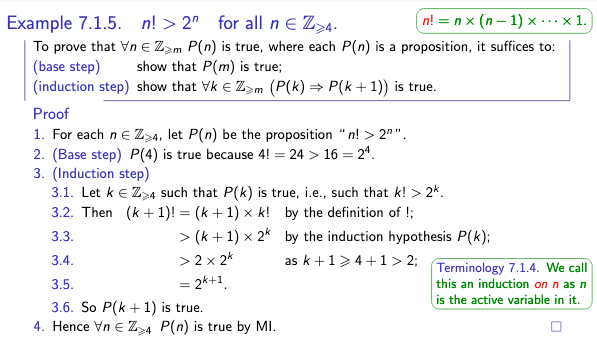
\includegraphics[width=12cm]{miexample.png}
    \end{center}

    \item Strong Mathematical Induction Example:
    
    \begin{center}
        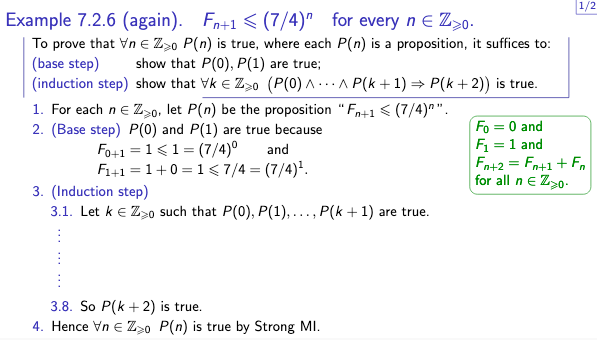
\includegraphics[width=12cm]{strongmiexample1.png}
        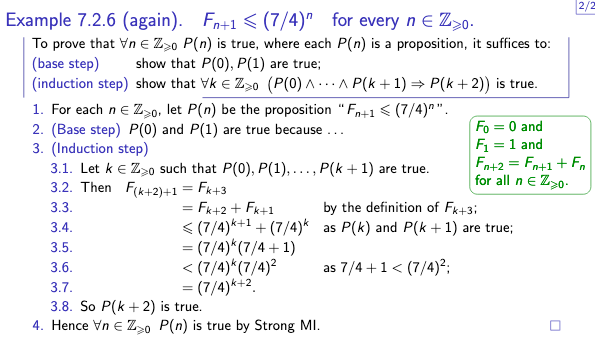
\includegraphics[width=12cm]{strongmiexample2.png}
    \end{center}

    \item Theorem 7.2.9 (Well-Ordering Principle): Every non-empty subset of $\mathbb{Z}_{\geqslant 0}$ has a smallest element.
    \item Recursive Definition consists of the base clause, recursion clause, and minimality clause.
    \item (Structural Induction over S, where S is a recursively defined set)
        \\ To prove that $\forall n\in S P(n)$ is true, where each $P(n)$ is a proposition, it suffices to:
        \\ \hspace*{3mm} (base step): show that $P(1)$ is true; and
        \\ \hspace*{3mm} (induction step): show that $\forall x\in S\ (P(x)\xrightarrow{} \{$recursive clause here\}) is true.  
\end{itemize}

% ==================================================
\section*{Divisibility, Primes and Base Expansion}
% ==================================================
\begin{itemize}
    \item Definition 8.1.1 (Divisibility $d|n$): Let $n,d\in \mathbb{Z}$. Then $d$ is said to divide $n$ if $n=dk$ for some $k\in \mathbb{Z}$. 
    \item Lemma 8.1.5: Let $n,d\in \mathbb{Z}$ with $d\neq 0$. Then $d|n$ if and only if $n/d\in \mathbb{Z}$.
    \item Lemma 8.1.9: Let $d,n\in \mathbb{Z}$. If $d|n$, then $-d|n$ and $d|{-n}$ and $-d|{-n}$.
    \item Proposition 8.1.10: Let $d,n\in \mathbb{Z}$. If $d|n$ and $n\neq 0$, then $|d|\leqslant|n|$.
    \item Theorem 8.1.12 (Transitivity of Divisibility): Let $a,b,c\in \mathbb{Z}$. If $a|b$ and $b|c$, then $a|c$.
    \item Lemma 8.1.14 (Closure Lemma of Division): Let $a,b,d,m,n\in \mathbb{Z}$. If $d|m$ and $d|n$, then $d|am+bn$.
    \item Theorem 8.1.16 (Division Theorem): For all $n\in \mathbb{Z}$ and $d\in \mathbb{Z}^+$, there exist unique $q,r\in \mathbb{Z}$ such that $n=dq+r$ and $0\leqslant r < d$.
        \\ (Note: $q$, the quotient is denoted by $n$ div $d$; $r$, the remainder is denoted by $n$ mod $d$)
        \\ \hspace*{3mm} - e.g. $11$ div $5 = 2$ and $11$ mod $5 = 1$ because $11 = 5\times 2 + 1$ and $0\leqslant 1 < 5$.
        \\ \hspace*{3mm} - e.g. $-16$ div $3=-6$ and $-16$ mod $3=2$ because $-16=3\times -6 + 2$ and $0\leqslant2 < 3$.
    \item Definition 8.2.1 (Primes and Composites):
        \\ \hspace*{3mm} (1) A positive integer is prime if it has exactly two positive divisors.
        \\ \hspace*{3mm} (2) A positive integer is composite if it has (strictly) more than two positive divisors.
    \item Lemma 8.2.4: An integer $n$ is composite if and only if $n$ has a divisor $d$ such that $1<d<n$.
    \item Lemma 8.2.5 (Prime Divisor Lemma): Let $n\in \mathbb{Z}_{\geqslant 2}$. Then $n$ has a prime divisor.
    \item Proposition 8.2.6: Let $n$ be a composite positive integer. Then $n$ has a prime divisor $p \leqslant \sqrt{n}$.
        \\ (Note: We can use the contraposition of Proposition 8.2.6 to prove that a number is a prime)
    \item Theorem 8.2.8 (Euclid): There are infinitely many prime numbers.
    \item Base-b Representation:
    
    \begin{center}
        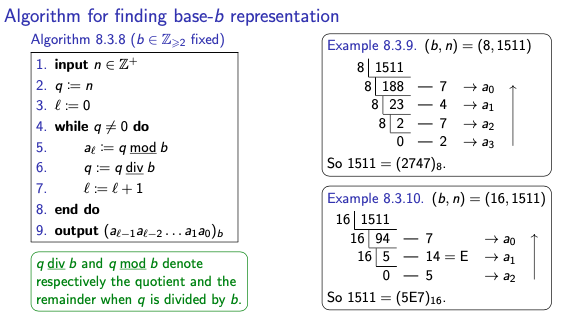
\includegraphics[width=12cm]{images/basebalgorithm.png}
        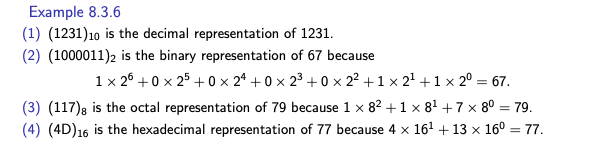
\includegraphics[width=12cm]{images/basebexample.png}
    \end{center}

    \item Tutorial 6 Q1: Let $a,b \in \mathbb{Z}$. If $a|b$ and $b|a$, then $a=b$ or $a=-b$.
    \item Tutorial 6 Q3: For all odd numbers $n \in \mathbb{Z}$, $n^2 div 4 = \frac{n^2 - 1}{4}$
    \item Tutorial 6 Q6: A positive integer $n$ is a perfect square $\xleftrightarrow{}$ $n$ has an odd number of positive divisors
    \item Tutorial 6 Q9: Let $n \in \mathbb{Z}_{\geqslant 1}$ with decimal representation $(a_\ell a_{\ell-1}...a_0)_{10}$. Then $9|n \xleftrightarrow{} 9|(a_0 + a_1 +...+ a_\ell)$
    \item Assignment 2 Q2: Let $a \in \mathbb{Z}_{\geq 2}$. Suppose that $\forall m,n \in \mathbb{Z}^+$, if $a|mn$, then $a|m$ or $a|n$. Then $a$ is prime.
\end{itemize}

% ==================================================
\section*{Euclidean Algorithm, Fundamental Theorem of Arithmetic and Modular Arithmetic}
% ==================================================
\begin{itemize}
    \item Definition 8.4.1 (gcd): Let $m,n\in \mathbb{Z}$.
        \\ \hspace*{3mm} (1) A common divisor of $m$ and $n$ is divisor of both $m$ and $n$.
        \\ \hspace*{3mm} (2) The greatest common divisor of $m$ and $n$ is denoted $gcd(m,n)$.
    \item Exercise 8.4.3: Let $m,n\in \mathbb{Z}^+$. $m$ mod $n=0$ if and only if $gcd(m,n)=n$.
    \item Exercise 8.4.6: Let $m,n\in \mathbb{Z}^+$. If $p$ is prime, then either $gcd(m,p)=1$ or $p|m$.
    \item Euclidean Algorithm (the divisor that gives remainder 0 is the gcd):

    \begin{center}
        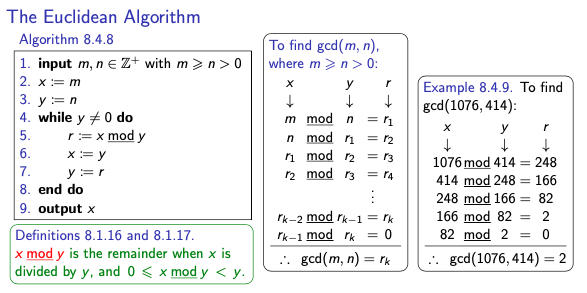
\includegraphics[width=12cm]{images/euclideanalgorithm.png}
    \end{center}

    \item Lemma 8.4.11: If $x,y,z\in \mathbb{Z}$ such that $x$ mod $y=r$, then $gcd(x,y)=gcd(y,r)$.
    \item Theorem 8.5.2 (Bezout's Lemma): For all $m,n\in \mathbb{Z}$ with $n\neq 0$, there exist $s,t\in \mathbb{Z}$ such that $gcd(m,n)=ms+nt$.
        \\ (Note: use the Euclidean Algorithm to backtrack and obtain this integer linear combination)
    \item Theorem 8.5.5 (Euclid's Lemma): Let $m,n,p\in \mathbb{Z}^+$. If $p$ is prime and $p|mn$, then $p|m$ or $p|n$.
    \item Corollary 8.5.6: Let $n,m_0,m_1,...,m_n,p\in \mathbb{Z}+$. If $p$ is prime and $p\ |\ m_0m_1...m_n$, then $p\ |\ m_i$ for some $i \in \{0,1,...,n\}$.
    \item Theorem 8.5.9 (Fundamental Theorem of Arithmetic; Prime Factorization Theorem):
        \\ Every integer $n\geqslant 2$ has a unique prime factorization in which the prime factors are arranged in nondecreasing order.
    \item Definition 8.6.1 (Congruence): Let $a,b\in \mathbb{Z}^+$. Then $a$ is congruent to $b$ modulo $n$ if $a$ mod $n$ = $b$ mod $n$. In this case, we write $a \equiv b$ (mod $n$).
    \item Lemma 8.6.2: The following are equivalent for all $a, b\in \mathbb{Z}$ and all $n\in \mathbb{Z}^+$:
        \\ \hspace*{3mm} (1) $a\equiv b$ (mod $n$)
        \\ \hspace*{3mm} (2) $a = nk + b$ for some $k\in \mathbb{Z}$
        \\ \hspace*{3mm} (3) $n\ |\ (a-b)$
    \item Lemma 8.6.5: Let $a,b,c\in \mathbb{Z}$ and $n\in \mathbb{Z}^+$:
        \\ \hspace*{3mm} (1) (Reflexivity) $a \equiv a$ (mod $n$)
        \\ \hspace*{3mm} (2) (Symmetry) If $a \equiv b$ (mod $n$), then $b \equiv a$ (mod $n$)
        \\ \hspace*{3mm} (3) (Transitivity) If $a\equiv b$ (mod $n$) and $b \equiv c$ (mod $n$), then $a\equiv c$ (mod $n$)
    \item Proposition 8.6.6 (Addition of Congruence): Let $a,b,c,d \in \mathbb{Z}$ and $n \in \mathbb{Z}^+$ such that $a\equiv b$ (mod $n$) and $c \equiv d$ (mod $n$). Then $a+c\equiv b + d$ (mod $n$).
    \item Proposition 8.6.13 (Multiplication of Congruence): Let $a,b,c,d\in \mathbb{Z}$ and $n\in \mathbb{Z}^+$ such that $a\equiv b$ (mod n) and $c\equiv d$ (mod $n$). Then $ac\equiv bd$ (mod $n$).
    \item Definition 8.6.8 (Additive Inverse): Let $a,b\in \mathbb{Z}$ and $n\in \mathbb{Z}^+$. The integer $b$ is an additive inverse of $a$ modulo $n$ if $a+b\equiv 0$ (mod $n$).
    \item Proposition 8.6.10 (Additive Inverse): Let $a,b\in \mathbb{Z}$ and $n\in \mathbb{Z}^+$.
        \\ \hspace*{3mm} (1) $-a$ is an additive inverse of $a$ modulo $n$.
        \\ \hspace*{3mm} (2) $b$ is an additive inverse of $a$ modulo $n$ if and only if $b \equiv -a$ (mod $n$).
    \item Definition 8.6.15 (Multiplicative Inverse): Let $a\in \mathbb{Z}$ and $n\in \mathbb{Z}^+$. A multiplicative inverse of $a$ modulo $n$ is an integer $b$ such that $ab\equiv 1$ (mod $n$).
    \item Proposition 8.6.16 (Multiplicative Inverse): Let $a\in \mathbb{Z}$ and $n\in \mathbb{Z}^+$.
        \\ \hspace*{3mm} (1) Let $b,b'$ be multiplicative inverses of $a$. Then $b\equiv b'$ (mod $n$).
        \\ \hspace*{3mm} (2) Let $b$ be a multiplicative inverse of $a$ and $b'\in \mathbb{Z}$ such that $b\equiv b'$ (mod $n$). Then $b'$ is also a multiplicative \hspace*{10mm}inverse of $a$.
    \item Theorem 8.6.19 (Existence of Multiplicative Inverse):
        \\ Let $a\in \mathbb{Z}$ and $n\in \mathbb{Z}^+$. Then $a$ has a multiplicative inverse modulo $n$ if and only if gcd($a$, $n$) $=1$.
        \\ (Note: Apply Bezout's Lemma to find Multiplicative Inverse, if it exists)
    \item Tutorial 7 Q2: Let $a,b,c \in \mathbb{Z}$ If $a\ |\ c$ and $b\ |\ c$ and $gcd(a,b)=1$, then $ab\ |\ c$.
    \item Tutorial 7 Q3: Let $a,b,s,t \in \mathbb{Z}$ such that $as+bt=1$. Then $gcd(a,b)=1$,
    \item Tutorial 7 Q4: Let $a,b,s,t \in \mathbb{Z}$ such that $as+bt=gcd(a,b)$. Then $gcd(s,t)=1$,
    \item Tutorial 7 Q5: Let $a,b \in \mathbb{Z}$ with $a\neq0$ or $b\neq0$. Then $gcd \left(\frac{a}{gcd(a,b)~}, \frac{b}{gcd(a,b)}\right) = 1$.
    \item Tutorial 7 Q6: Let $a,b \in \mathbb{Z}$ with $a\neq0$ or $b\neq0$. Then an integer $n$ is an integer linear combination of $a$ and $b \xleftrightarrow{} gcd(a,b)\ |\ n$.
\end{itemize}

% ==================================================
\section*{Relations, Equivalence Relations and Partitions, and Partial Orders}
% ==================================================
\begin{itemize}
    \item Definition 9.1.1 (Relations): 
        \\ \hspace*{3mm} (1) A relation from $A$ to $B$ is a subset of $A \times B$.
        \\ \hspace*{3mm} (2) Let $\mathrel{R}$ be a relation from $A$ to $B$ and $(x,y)\in A\times B$. Then we may write:
        \begin{center}
            $x \mathrel{R} y$ for $(x,y)\in R$ \ and \  $x \centernot{R} y$ for $(x, y) \not\in \mathrel{R}$\\
        \end{center}
        \hspace*{3mm} (3) $R^{-1}$ is the inverse relation of $R$ (i.e. $R^{-1}=\{(y,x):(x,y)\in R\}$)
    \item Definition 9.2.1: A (binary) relation on a set $A$ is a relation from $A$ to $A$.
    \item Definition 9.2.2: Let $A$ be a set and $R$ be a relation on $A$.
        \\ \hspace*{3mm} (1) $R$ is reflextive if $\forall x\in A\ (x \mathrel{R} x)$
        \\ \hspace*{3mm} (2) $R$ is symmetric if $\forall x,y\in A\ (x \mathrel{R} y \xrightarrow{} y \mathrel{R} x)$
        \\ \hspace*{3mm} (3) $R$ is transitive if $\forall x,y,z\in A\ (x \mathrel{R} y \land  y \mathrel{R} z \xrightarrow{} x \mathrel{R} z)$
    \item Definition 9.2.9 (Equivalence Relations): An equivalence relation is a relation that is reflexive, symmetric and transitive
    \item Definition 9.2.10 (Equivalence Class): Let $A$ be a set and $R$ be an equivalence relation on $A$. For each $x\in A$, the equivalence class of $x$ with respect to $R$, denoted $[x]_R$, is defined by:
        \begin{equation*}
            [x]_R=\{y\in A: x \mathrel{R} y\}
        \end{equation*}
    \item $A/R = \{[x]_R:x\in A\}$
    \item Proposition 9.2.13: Let $R$ be an equivalence relation on a set $A$. The following are equivalent for all $x,y\in A$:
        \\ \hspace*{3mm} (1) $x\mathrel{R}y$
        \\ \hspace*{3mm} (2) $[x]=[y]$
        \\ \hspace*{3mm} (3) $[x]\cap[y]\neq \varnothing$
    \item Definition 9.3.1 (Partitions): A partition of a set $A$ is a set $C$ of nonempty subsets of $A$ such that
        \\ \hspace*{3mm} $(\geqslant 1)\ \ \forall x\in A\ \exists S\in C\ (x\in S)$ and
        \\ \hspace*{3mm} $(\leqslant 1)\ \ \forall x\in A\ \forall S,S'\in C\ (x\in S \land x\in S' \xrightarrow{} S=S')$
        \\ (Note: elements of a partition are called components of the partition.)
    \item Theorem 9.3.4: Let $R$ be an equivalence relation on a set $A$. Then $A/R$ is a partition on $A$.
    \item Theorem 9.3.5: Let $C$ be a partition of a set $A$. Then there is an equivalence relation $R$ on $A$ such that $A/R=C$.
    \item Definition 9.4.1 (Partial Orders): Let $A$ be a set and $R$ be a relation on $A$.
        \\ \hspace*{3mm} (1) $R$ is antisymmetric if $\forall x,y\in A\ (x\mathrel{R}y\land y\mathrel{R}x \xrightarrow{} x=y)$
        \\ \hspace*{3mm} (2) $R$ is a (non-strict) partial order if $R$ is reflexive, antisymmetric, and transitive
        \\ \hspace*{3mm} (3) $R$ is a (non-strict) total order if $R$ is a partial order and $\forall x,y\in A\ (x\mathrel{R}y \lor y\mathrel{R}x)$
    \item Hasse Diagrams:
        \begin{center}
            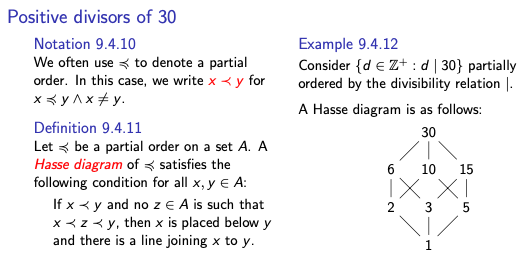
\includegraphics[width=12cm]{images/hassediagram.png}
        \end{center}
    \item Definition 9.5.1 Let $\preccurlyeq$ be a partial order on a set $A$, and $c\in A$:
        \\ \hspace*{3mm} (1) $c$ is a minimal element if $\forall x\in A\ (x\preccurlyeq c \xrightarrow{}c=x)$
        \\ \hspace*{3mm} (2) $c$ is a maximal element if $\forall x\in A\ (c \preccurlyeq x \xrightarrow{} c=x)$
        \\ \hspace*{3mm} (3) $c$ is the smallest element (or the minimum element) if $\forall x\in A\ (c \preccurlyeq x)$
        \\ \hspace*{3mm} (4) $c$ is the largest element (or the maximum element) if $\forall x\in A\ (x \preccurlyeq c)$
    \item Lemma 9.5.5: Consider a partial order $\preccurlyeq$ on a set $A$.
        \\ \hspace*{3mm} (1) A smallest element. is minimal
        \\ \hspace*{3mm} (2) There is at most one smallest element.
    \item Proposition 9.5.7: With respect to any partial order $\preccurlyeq$ on a finite set $A\neq \varnothing$, one can find a minimal element.
    \item Theorem 9.5.9: Let $A$ be a set and $\preccurlyeq$ be a partial order on $A$. Then there exists a total order $\preccurlyeq^*$ on $A$ such that for all $x,y\in A,\ x\preccurlyeq y \xrightarrow{} x\preccurlyeq^* y$
    \item (Linearization) Just use the $\leqslant$ total order for linearization. But where $\leqslant$ is not possible:
        \begin{center}
            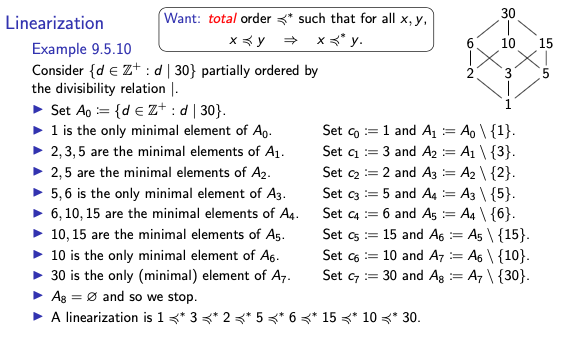
\includegraphics[width=12cm]{images/linearization.png}
        \end{center}
    \item Tutorial 8 Q2: Let $R$ be a relation on a set A. $R$ is symmetric $\xleftrightarrow{} R=R^{-1}$
    \item Tutorial 8 Q5: Let $A,B$ be non-empty sets and $f$ be a surjection $A \xrightarrow{} B$. Then $C = \{\{x \in A : f(x)=y\}:y \in B\}$ is a partition on A.
    \item Assignment 2 Q5: Let $C$ be a partition on a set $A$. Then there exists a set $B$ and a surjection $f : A \xrightarrow{} B$ such that $C = \{\{x \in A : f(x)=y\} : y \in B\}$.
\end{itemize}

% ==================================================
\section*{Counting and Probability I}
% ==================================================
\begin{itemize}
    \item Theorem 9.1.1 (The Number of Elements in a List): If $m$ and $n$ are integers and $m\leqslant n$, then there are $n-m+1$ integers from $m$ t $n$ inclusive.
    \item Theorem 9.2.1 (Multiplication/ Product Rule): If an operation consists of $k$ steps and
        \\ \hspace*{5mm} the first step can be performed in $n_1$ ways,
        \\ \hspace*{5mm} the second step can be performed in $n_2$ ways (regardless of how the first step was performed),
        \\ \hspace*{5mm} ...
        \\ \hspace*{5mm} the $k^{th}$ step can be performed in $n_k$ ways (regardless of how the preceding steps were performed),
        \\ Then the entire operation can be performed in $n_1\times n_2\times ...\times n_k$ ways.
    \item Theorem 9.2.2 (Permutations): The number of permutations of a set with $n\ (n\geqslant 1)$ elements is $n!$.
    \item Theorem 9.2.3 ($r$-permutations from a set of $n$ elements): If $n$ and $r$ are integers and $1\leqslant r\leqslant n$, then the number of $r$-permutations of a set of $n$ elements is given by the formula:
        \begin{equation*}
            P(n,r) = n(n-1)(n-2)...(n-r+1) = \frac{n!}{(n-r)!}
        \end{equation*}
    \item Theorem 9.3.1 (The Addition/ Sum Rule): Suppose a finite set $A$ equals the union of $k$ distinct mutually disjoint subsets $A_1,A_2,...,A_k$. Then $|A|=|A_1|+|A_2|+...+|A_k|$.
    \item Theorem 9.3.2 (The Difference Rule): If $A$ is a finite set and $B \subseteq A$, then $|A\backslash B|=|A|-|B|$.
    \item Formula for the Probability of the Complement of an Event: $P(\bar{A})=1-P(A)$
    \item Theorem 9.3.3 (The Inclusion/ Exclusion Rule): If $A$, $B$, and $C$ are any finite sets, then:
        \\ \hspace*{3mm} (1) $|A\cup B|=|A|+|B|-|A\cap B|$
        \\ \hspace*{3mm} (2) $|A\cup B\cup C|=|A|+|B|+|C|-|A\cap B|-|A\cap C|-|B\cap C|+|A\cap B\cap C|$
    \item (Pigeonhole Principle): A function from one finite set to a smaller finite set cannot be one-to-one: There must be at least 2 elements in the domain that have the same image in the co-domain.
    \item (Generalized Pigeonhole Principle): For any function $f$ from a finite set $X$ with $n$ elements to a finite set $Y$ with $m$ elements and for any positive integer $k$, if $k<n/m$, then there is some $y\in Y$ such that $y$ is the image of at least $k+1$ distinct elements of $X$.
        \smallskip
        \\ \hspace*{3mm} e.g. to fit 28 pigeons into 9 pigeonholes, it is guaranteed that some hole has 4 pigeons since $k=3<28/9$ and \hspace*{10mm} $k+1=4$
        \smallskip
        \\(Contrapositive Form): For any function $f$ from a finite set $X$ with $n$ elements to a finite set $Y$ with $m$ elements and for any positive integer $k$, if for each $y\in Y,\  f^{-1}(\{y\})$ has at most $k$ elements, then $X$ has at most $km$ elements; in other words, $n\leqslant km$.
        \smallskip
        \\ \hspace*{3mm} e.g. If there are 10 modules, and each module is attended by at most 1000 students, then the total number \hspace*{10mm} of students is at most 10000
\end{itemize}

% ==================================================
\section*{Counting and Probability II}
% ==================================================
\begin{itemize}
    \item (Combinations): An $r$-combination of a set of $n$ elements is a subset of $r$ of the $n$ elements. $\binom{n}{r}$ denotes the number of subsets of size $r$ ($r$-combinations) that can be chosen from a set of $n$ elements.
    \item Theorem 9.5.1 (Formula for $\binom{n}{r}$):
        \begin{equation*}
            \binom{n}{r}= \frac{P(n,r)}{r!} = \frac{n!}{r!(n-r)!}\ ,\ \text{where}\ n\ \text{and}\ r\ \text{are non-negative integers with}\ r\leqslant n.
        \end{equation*}
    \item Theorem 9.5.2 (Permutations with Sets of Indistinguishable Objects): 
        \begin{equation*}
            \frac{n!}{n_1!n_2!...n_k!}\ ,\ \text{where}\ n_1, n_2, ..., n_k\ \text{are the number of objects of type}\ 1, 2, ...,k
        \end{equation*}
    \item Theorem 9.6.1 (Number of $r$-combinations with Repetition Allowed/ Number of multisets of size $r$):
        \begin{equation*}
            \binom{r+n-1}{r}\ ,\ \text{where}\ r\ \text{is the number of objects to be selected from a set of}\ n\ \text{elements}
        \end{equation*}
        \\ (This equals the number of ways $r$ objects can be selected from $n$ categories of objects with repetitions allowed. Or similarly, $r$ number of objects, and $n-1$ 'category dividers')
    \item Theorem 9.7.1 (Pascal's Formula):
        \begin{equation*}
            \binom{n+1}{r} = \binom{n}{r-1} + \binom{n}{r}\ ,\ \text{where}\ n,r\in \mathbb{Z}^+\ \text{and}\ r\leqslant n
        \end{equation*}
    \item Lecture Example 8: $\binom{n}{r}=\binom{n}{n-r}$
    \item Lecture Example 10: $k\binom{n}{k}=n\binom{n-1}{k-1}$
    \item Theorem 9.7.2 (Binomial Theorem): Given any real numbers $a$ and $b$ and any non-negative integer $n$,
        \begin{equation*}
            (a+b)^n=\Sigma^n_{k=0}\binom{n}{k}a^{n-k}b^k = a^n+\binom{n}{1}a^{n-1}b^1+\binom{n}{2}a^{n-2}b^2+...+\binom{n}{n-1}a^1b^{n-1}+b^n
        \end{equation*}
    \item (Probability Axioms):
        \\ \hspace*{3mm} (1) $0\leqslant P(A)\leqslant1$, where $A$ is an event in sample space $S$
        \\ \hspace*{3mm} (2) $P(\varnothing)=0$ and $P(S)=1$
        \\ \hspace*{3mm} (3) If $A$ and $B$ are disjoint events $(A\cap B=\varnothing)$, then $P(A\cup B)=P(A)+P(B)$
    \item (Probability of the Complement of an Event): If $A$ is any event in a sample space $S$, then $P(\bar{A})=1-P(A)$
    \item (Probability of a General Union of Two Events): If $A$ and $B$ are any events in a sample space $S$, then $P(A\cup B)=P(A)+P(B)-P(A\cap B)$.
    \item (Expected Value): Suppose the possible outcomes of an experiment, or random process, are real numbers $a_1,a_2,...,a_n$ which occur with probabilities $p_1,p_2,...,p_n$ respectively. The expected value of the process is:
        \begin{equation*}
            \Sigma^n_{k=1}a_kp_k=a_1p_1+a_2p_2+...+a_np_n
        \end{equation*}
    \item (Linearity of Expectation): The expected value of the sum of random variables is equal to the sum of their individual expected values, regardless of whether they are independent.
        \smallskip
        \\ \hspace*{3mm} For random variables $X$ and $Y$ (which may be dependent), $E[X+Y]=E[X]+E[Y]$
        \smallskip
        \\ \hspace*{3mm} e.g. Using linearity of expectation, the expected value for the sum of two dice = $3.5+3.5=7$, where 3.5 is \hspace*{3mm} the expected value for a fair dice
    \item (Conditional Probability): Let $A$ and $B$ be events in a sample space $S$. If $P(A)\neq0$, then the conditional probability of $B$ given $A$ is:
        \\ \hspace*{3mm} (1) $P(B|A)=\frac{P(A\cap B)}{P(A)}$
        \\ \hspace*{3mm} (2) $P(A\cap B)=P(B|A)\cdot P(A)$
        \\ \hspace*{3mm} (3) $P(A)=\frac{P(A\cap B)}{P(B|A)}$
    \item Theorem 9.9.1 (Bayes' Theorem):
        \begin{equation*}
            P(B_k|A) = \frac{P(A|B_k)\cdot P(B_k)}
            {P(A|B_1)\cdot P(B_1)+P(A|B_2)\cdot P(B_2)+...+P(A|B_n)\cdot P(B_n)}\ ,
        \end{equation*}
        \begin{center}
            where $B_1, B_2,...B_n$ are mutually disjoint events, and $A$ and all the $B_i$ have non-zero probabilities
        \end{center}
    \item (Independent Events): If $A$ and $B$ are events in a sample space $S$, then $A$ and $B$ are independent if and only if:
        \begin{equation*}
            P(A\cap B)=P(A)\cdot P(B)
        \end{equation*}
    \item (Pairwise Independent and Mutually Independent) Three events $A$, $B$, and $C$ are pairwise independent, if and only if, they satisfy conditions 1-3 below. They are mutually independent, if and only if, they satisfy all four conditions below:
        \smallskip
        \\ \hspace*{3mm} (1) $P(A\cap B)=P(A)\cdot P(B)$
        \\ \hspace*{3mm} (2) $P(A\cap C)=P(A)\cdot P(C)$
        \\ \hspace*{3mm} (3) $P(B\cap C)=P(B)\cdot P(C)$
        \\ \hspace*{3mm} (4) $P(A\cap B\cap C)=P(A)\cdot P(B)\cdot P(C)$
        \smallskip
        \\ (Note: Events can be pairwise independent without satisfying the condition $P(A\cap B\cap C)=P(A)\cdot P(B)\cdot P(C)$. Conversely, they can satisfy the condition $P(A\cap B\cap C)=P(A)\cdot P(B)\cdot P(C)$ without being pairwise independent.)
    \item (Generalized Definition of Mutually Independent): Events $A_1, A_2,...,A_n$ in a sample space $S$ are mutually independent, if and only if, the probability of the intersection of any subset of the events is the product of the probabilities of the events in the subset.
\end{itemize}

% ==================================================
\section*{Graphs}
% ==================================================
\begin{itemize}
    \item (Simple Graph): A simple graph is an undirected graph that does not have any loops or parallel edges. (That is, there is at most one edge between each pair of distinct vertices.)
    \item (Complete Graphs): A complete graph on $n$ vertices, $n>0$, denoted $K_n$, is a simple graph with $n$ vertices and exactly one edge connecting each pair of distinct vertices.
    \item (Bipartite Graph): A bipartite graph (or bigraph) is a simple graph whose vertices can be divided into two disjoint sets $U$ and $V$ such that every edge connects a vertex in $U$ to one in $V$.
    \item (Complete Bipartite Graph): A complete bipartite graph is a bipartite graph on two disjoint sets $U$ and $V$ such that every vertex in $U$ connects to every vertex in $V$.
        \\ (Note: If $|U|=m$ and $|V|=n$, the complete bipartite graph is denoted as $K_{m,n}$)
    \item (Subgraph of a Graph): A graph $H$ is said to be a subgraph of graph $G$ if and only if every vertex in $H$ is also a vertex in $G$, every edge in $H$ is also an edge in $G$, and every edge in $H$ has the same endpoints as it has in $G$.
    \item (Degree of a Vertex and Total Degree of an Undirected Graph):
        \smallskip    
        \\ \hspace*{3mm} (1) Let $G$ be an undirected graph and $v$ a vertex of $G$. The degree of $v$, denoted deg($v$), equals the number \hspace*{9mm} of edges that are incident on $v$, with an edge that is a loop counted twice.
        \smallskip
        \\ \hspace*{3mm} (2) The total degree of $G$ is the sum of the degrees of all the vertices of $G$.
    \item Theorem 10.1.1 (The Handshake Theorem): The total degree of a graph $G=2\times$ (the number of edges of $G$)
    \item Corollary 10.1.2: The total degree of a graph is even.
    \item Proposition 10.1.3: In any graph there are an even number of vertices of odd degree.
    \item (Walk): A walk from $v$ to $w$ is a finite alternating sequence of adjacent vertices and edges of $G$.
    \item (Trivial Walk): The trivial walk from $v$ to $v$ consists of the single vertex $v$.
    \item (Trail): A trail from $v$ to $w$ is a walk from $v$ to $w$ that does not contain a repeated edge.
    \item (Path): A path from $v$ to $w$ is a trail that does not contain a repeated vertex.
    \item (Closed Walk): A closed walk is a walk that starts and ends at the same vertex.
    \item (Circuit/ Cycle): Let $n\in \mathbb{Z}_{\geqslant 3}$. An undirected graph $G(V, E)$ where 
        \begin{equation*}
            V=\{x_1,x_2,...,x_n\}\ \text{and}\ E=\{\{x_1,x_2\},\{x_2,x_3\},...,\{x_{n-1},x_n\},\{x_n,x_1\}\}
        \end{equation*}
        is called a circuit/ cycle. (AKA: a circuit is a closed walk that does not contain a repeated edge)
    \item (Simple Circuit): A simple circuit (or simple cycle) is a circuit that does not have any other repeated vertex except the first and last.
    \item An undirected graph is cyclic if it contains a loop or a cycle; otherwise, it is acyclic.
    \item (Connectedness): A graph $G$ is connected if and only if given any two vertices $v$ and $w$ in $G$, there is a walk from $v$ to $w$.
    \item Lemma 10.2.1: Let $G$ be a graph.
        \\ \hspace*{2.5mm} (1) If $G$ is connected, then any two distinct vertices of $G$ can be connected by a path.
        \\ \hspace*{2.5mm} (2) If vertices $v$ and $w$ are part of a circuit in $G$ and one edge is removed from the circuit, then there still \hspace*{8.5mm} exists a trail from $v$ to $w$ in $G$.
        \\ \hspace*{3mm} (3) If $G$ is connected and $G$ contains a circuit, then an edge of the circuit can be removed without disconnecting \hspace*{8.5mm} $G$.
    \item (Connected Component): A graph $H$ is a connected component of a graph $G$ if and only if
        \\ \hspace*{3mm} (1) The graph $H$ is a subgraph of $G$.
        \\ \hspace*{3mm} (2) The graph $H$ is connected.
        \\ \hspace*{3mm} (3) No connected subgraph of $G$ has $H$ as a subgraph and contains vertices or edges that are not in $H$.
        \\ (AKA: a connected component of a graph is a connected subgraph of largest possible size)
    \item (Euler Circuit): Let $G$ be a graph. An Euler Circuit for $G$ is a circuit that contains every vertex and traverses every edge of $G$ exactly once.
    \item (Eulerian Graph): An Eulerian Graph is a graph that contains an Euler Circuit.
    \item Theorem 10.2.2: If a graph has an Euler Circuit, then every vertex of the graph has positive even degree.
        \\ (Contrapositive): If some vertex of a graph has odd degree, then the graph does not have an Euler Circuit.
    \item Theorem 10.2.3: If a graph $G$ is connected and the degree of every vertex of $G$ is a positive even integer, then $G$ has an Euler Circuit.
    \item Theorem 10.2.4: A graph $G$ has an Euler Circuit if and only if $G$ is connected and every vertex of $G$ has positive even degree.
    \item (Euler Trail): An Euler Trail from $v$ to $w$ is a sequence of adjacent edges and vertices that starts at $v$, ends at $w$, passes through every vertex of $G$ at least once, and traverses every edge of $G$ exactly once.
    \item Corollary 10.2.5: There is an Euler Trail from $v$ to $w$ if and only if $G$ is connected, $v$ and $w$ have odd degree, and all other vertices of $G$ have positive even degree.
    \item (Hamiltonian Circuit): A Hamiltonian Circuit for $G$ is a simple circuit that includes every vertex of $G$. (That is, every vertex appears exactly once, except for the first and the last, which are the same.)
    \item (Hamiltonian Graph): A Hamiltonian Graph is a graph that contains a Hamiltonian Circuit.
    \item (Differences between Euler Circuit and Hamiltonian Circuit):
        \\ \hspace*{3mm} (1) Euler Circuit may visit some vertices more than once while Hamiltonian Circuit can only visit each vertex \hspace*{8.7mm} exactly once (both visit all vertices in $G$)
        \\ \hspace*{3mm} (2) Euler Circuit traverses every edge in $G$ exactly once, while Hamiltonian Circuit does not need to traverse \hspace*{8.7mm} all edges.
    \item Proposition 10.2.6: If a graph $G$ has a Hamiltonian Circuit, then $G$ has a subgraph $H$ with the following properties:
        \\ \hspace*{3mm} (1) $H$ contains every vertex of $G$
        \\ \hspace*{3mm} (2) $H$ is connected
        \\ \hspace*{3mm} (3) $H$ has the same number of edges as vertices
        \\ \hspace*{3mm} (4) Every vertex of $H$ has degree 2
        \\ (Contraposition): If a graph $G$ does not have a subgraph $H$ with properties (1)-(4), then $G$ does not have a \hspace*{27.5mm}  Hamiltonian Circuit
    \item Adjacency Matrix (Directed and Undirected Graphs):
        \begin{center}
            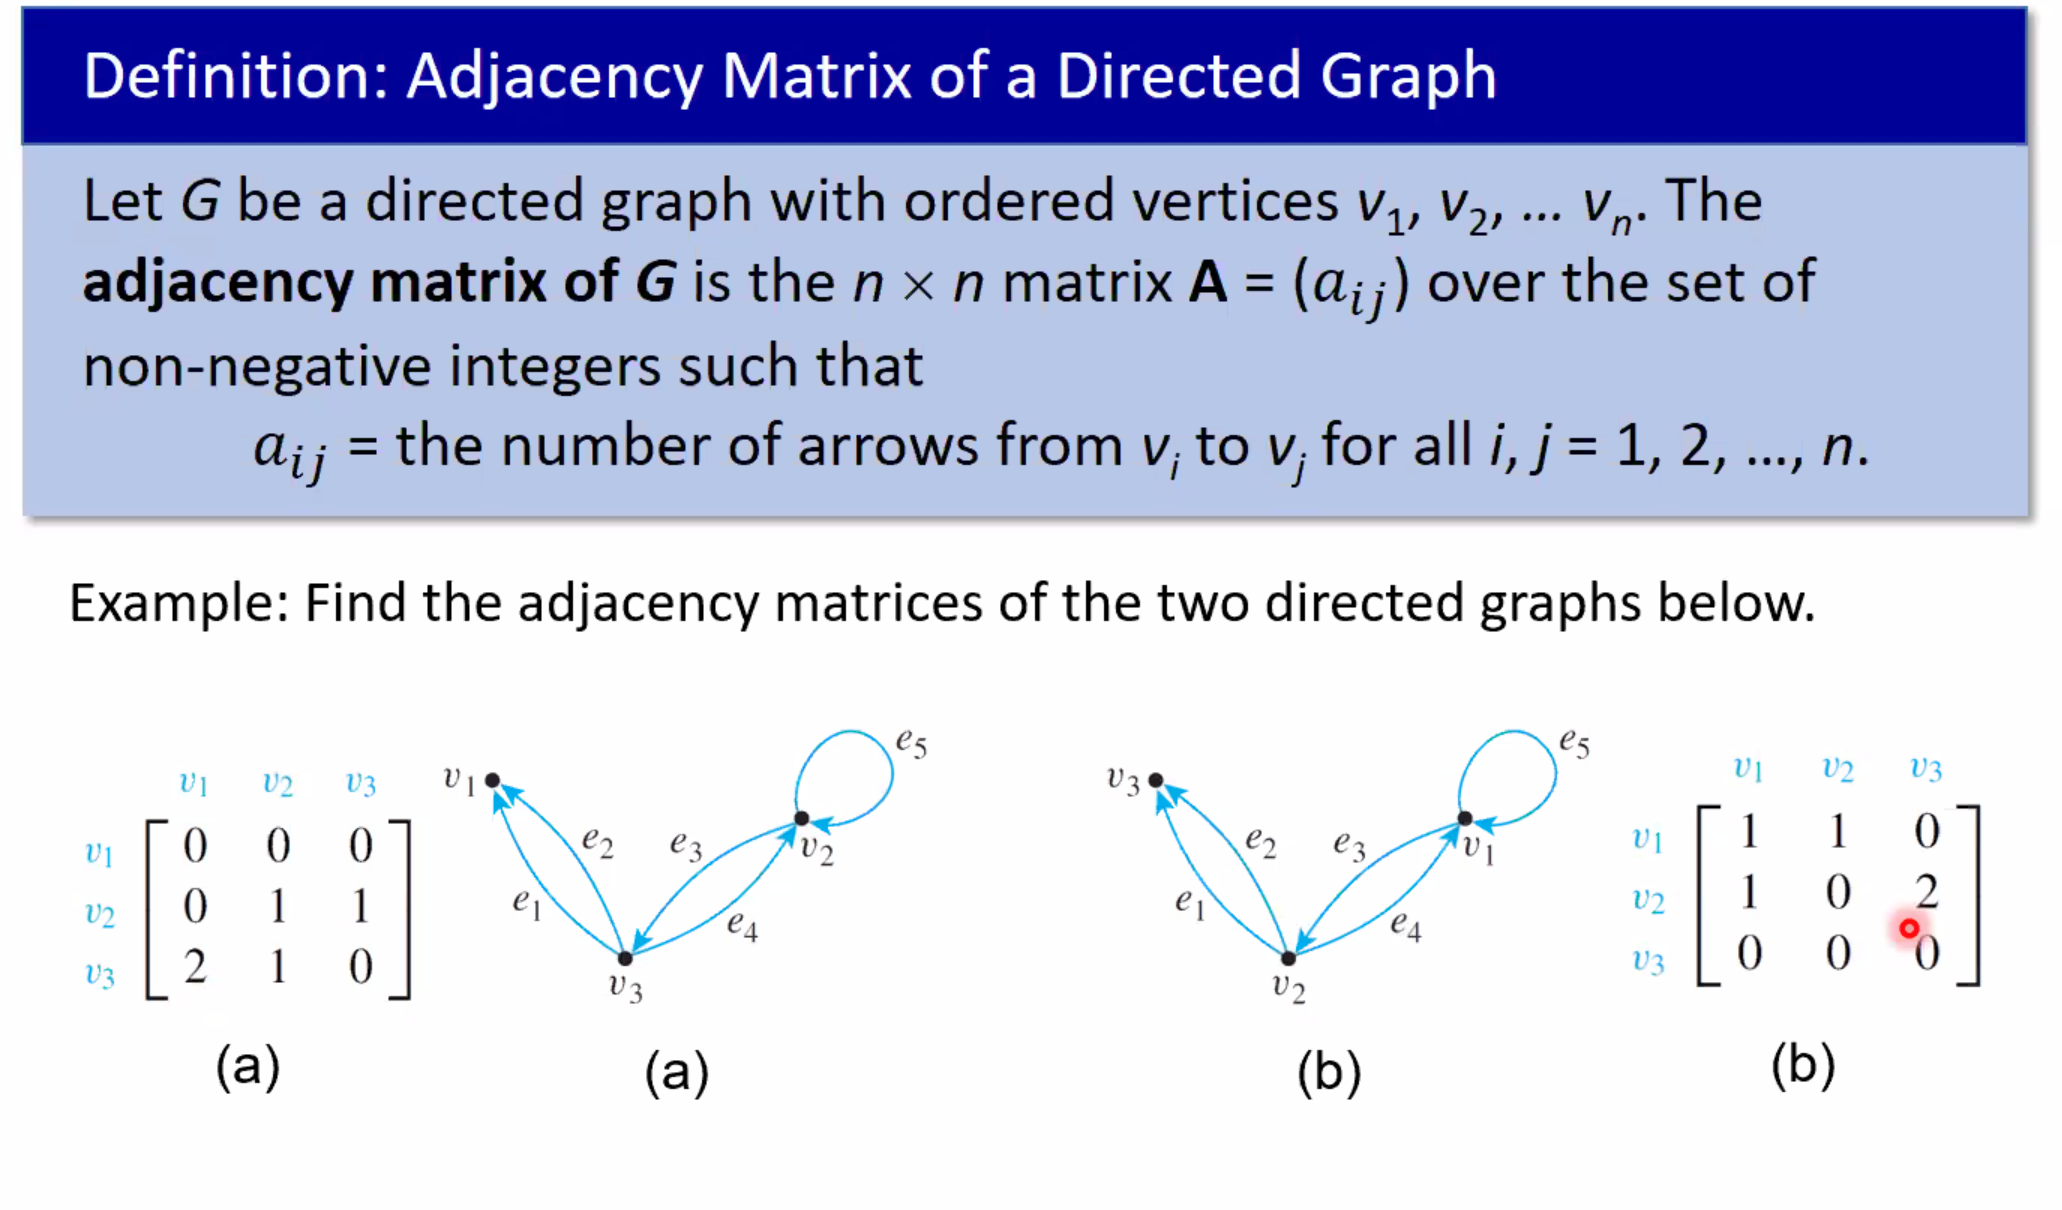
\includegraphics[width=8cm]{adjacencymatrixdirectedgraph.png}
            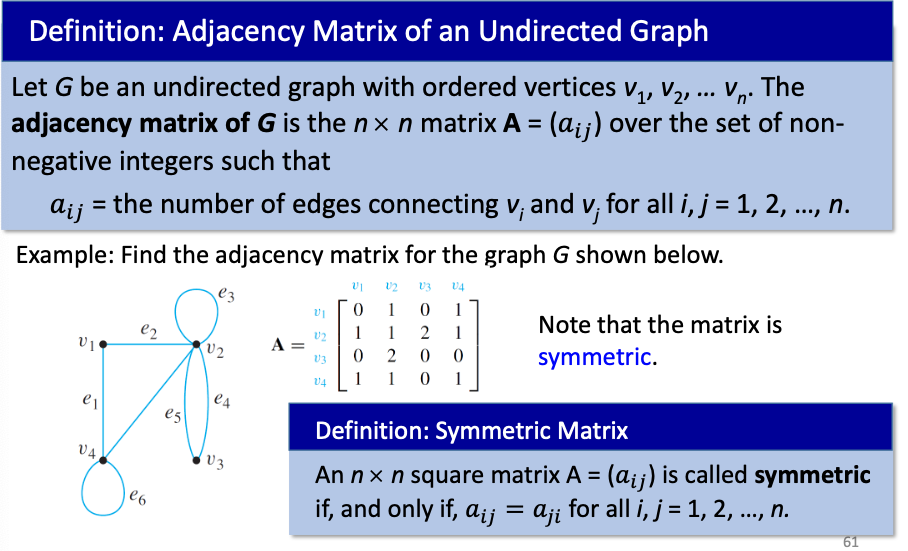
\includegraphics[width=8cm]{adjacencymatrixundirectedgraph.png}
        \end{center}
    \item Theorem 10.3.2 (n-th power of adjacency matrix): The ij-th entry of $A^n=$ the number of walks of length $n$ from $v_i$ to $v_j$ 
    \item (Isomorphic Graph): Let $G=(V_G, E_G)$ and $G'=(V_{G'}, E_{G'})$ be two graphs.
        \\ $G$ is isomorphic to $G'$ if and only if there exists a permutation $\pi: V_G \xrightarrow{} V_{G'}$ such that $\{u,v\}\in E_G \xleftrightarrow{} \{\pi (u),\pi(v)\}\in E_{G'}$.
    \item Theorem 10.4.1: Let $S$ be a set of graphs and let $\cong$ be the relation of graph isomorphism on $S$. Then $\cong$ is an equivalence relation on $S$.
    \item (Planar Graph): A planar graph is a graph that can be drawn on a (two-dimensional) plane without edges crossing.
    \item Kuratowski's Theorem: A finite graph is planar if and only if it does not contain a subgraph that is a subdivision of the complete graph $K_5$ or the complete bipartite graph $K_{3,3}$.
    \item Euler's Formula: For a connected planar simple graph $G=(V,E)$ with $e=|E|$ and $v=|V|$, if we let $f$ be the number of faces, then $f=e-v+2$
    \item Tutorial 11 Q2: Every simple graph with at least two vertices has two vertices of the same degree.
    \item Tutorial 11 Q4: For any simple graph with 6 vertices, $G$ or its complementary graph contains a triangle.
    \item Tutorial 11 Q6: There are $v - k$ edges in a forest (where $v$ is the number of vertices and $k$ is the number of components).
    \item Tutorial 11 Q8a: If $G$ is a complete graph with n vertices, the total number of spanning trees in $G$ is $n^{n-2}$.
\end{itemize}

% ==================================================
\section*{Trees}
% ==================================================
\begin{itemize}
    \item (Tree): A graph is called a tree if and only if it is circuit-free and connected.
    \item (Trivial Tree): A trivial tree is a graph that consists of a single vertex.
    \item (Forest): A graph is called a forest if and only if it is circuit-free and not connected.
    \item Lemma 10.5.1: Any non-trivial tree has at least one vertex of degree 1.
    \item (Terminal Vertex/ leaf and internal vertex): 
        \\ \hspace*{3mm} (1) If $T$ has only one or two vertices, then each is called a terminal vertex (or leaf).
        \\ \hspace*{3mm} (2) If $T$ has at least three vertices, then a vertex of degree 1 in $T$ is called a terminal vertex (or leaf), and a \hspace*{9mm} vertex of degree greater than 1 in $T$ is called an internal vertex.
    \item Theorem 10.5.2: Any tree with $n$ vertices $(n>0)$ has $n-1$ edges.
    \item Lecture Example: A non-trivial tree has at least 2 vertices of degree 1.
    \item Lemma 10.5.3: If $G$ is any connected graph, $C$ is any circuit in $G$, and one of the edges of $C$ is removed from $G$, then the graph that remains is still connected.
    \item Theorem 10.5.4: If $G$ is a connected graph with $n$ vertices and $n-1$ edges, then $G$ is a tree.
    \item (Rooted Trees): A rooted tree is a tree in which there is one vertex that is distinguished from the others and is called the root.\\ (Level): The level of a vertex is the number of edges along the unique path between it and the root.\\ (Height): The height of a rooted tree is the maximum level of any vertex of the tree.\\(Also know: children, parent, siblings, ancestor, descendant)
    \item (Binary Tree): A binary tree is a rooted tree in which every parent has at most two children (a left child, a right child or both)
    \item (Full Binary Tree): A full binary tree is a binary tree in which each parent has exactly two children. \\(Also know what is Left Subtree and Right Subtree of a (Full) Binary Tree)
    \item Theorem 10.6.1 (Full Binary Tree Theorem): If $T$ is a full binary tree with $k$ internal vertices, then $T$ has a total of $2k+1$ vertices and has $k+1$ terminal vertices (leaves).
    \item Theorem 10.6.2: For non-negative integers $h$, if $T$ is any binary tree with height $h$ and $t$ terminal vertices (leaves), then $t\leqslant 2^h$. Equivalently, $log_2t\leqslant h$
    \pagebreak
    \item Binary Tree Traversal:
        \begin{center}
            \raisebox{0.19\height}{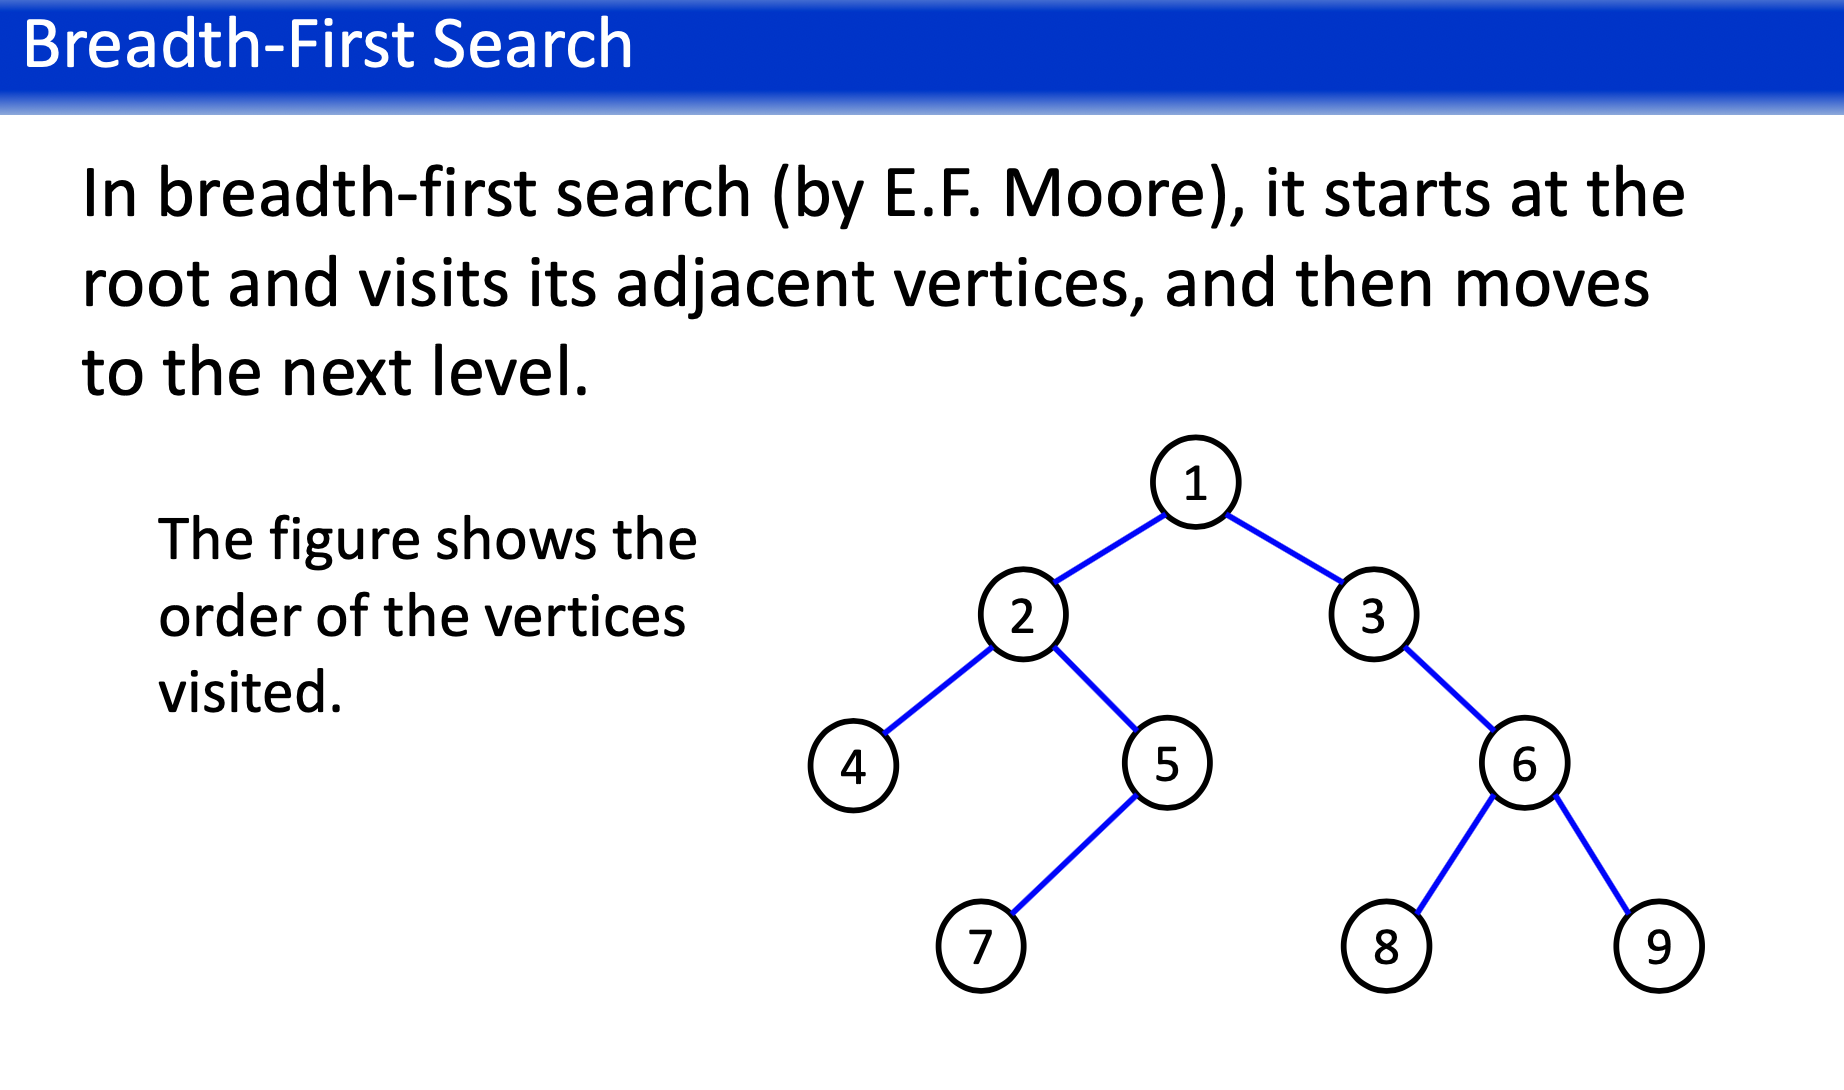
\includegraphics[width=8cm]{images/bfs.png}}
            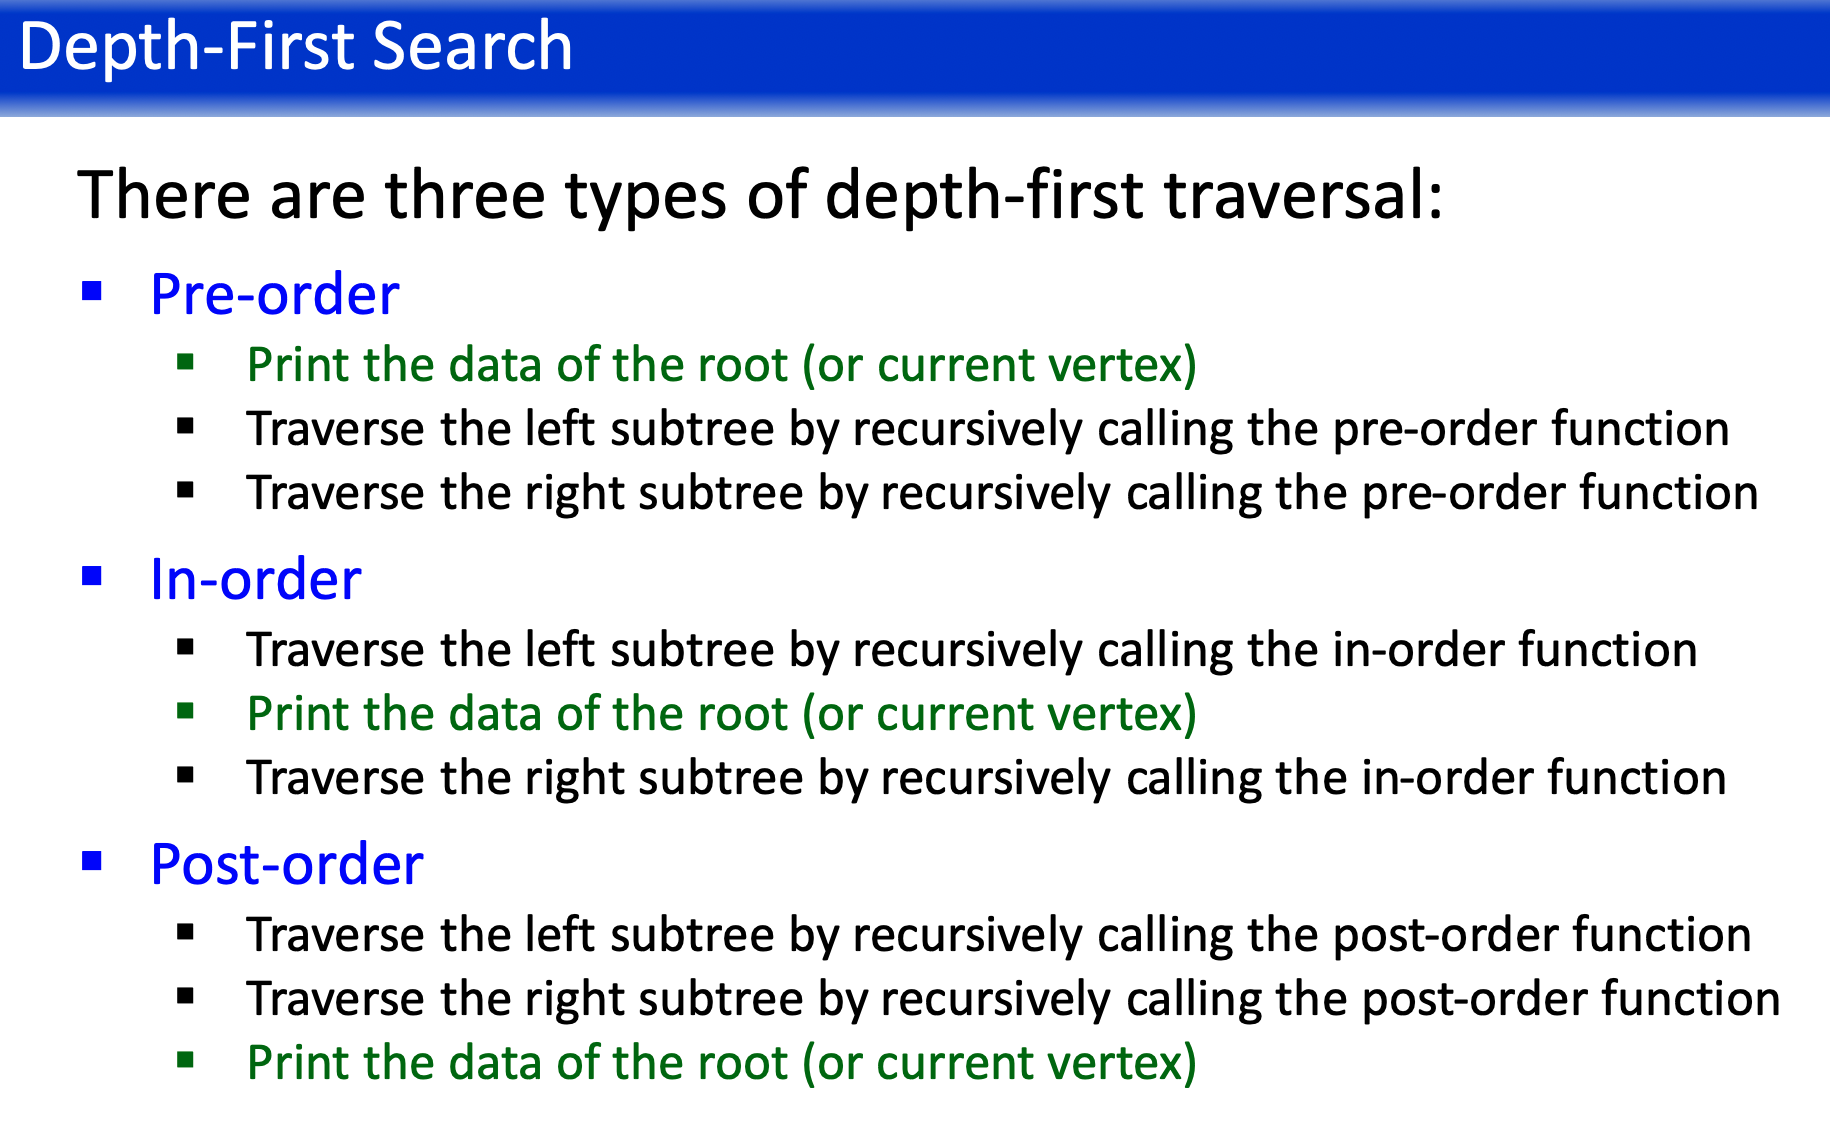
\includegraphics[width=9cm]{images/dfs.png}
            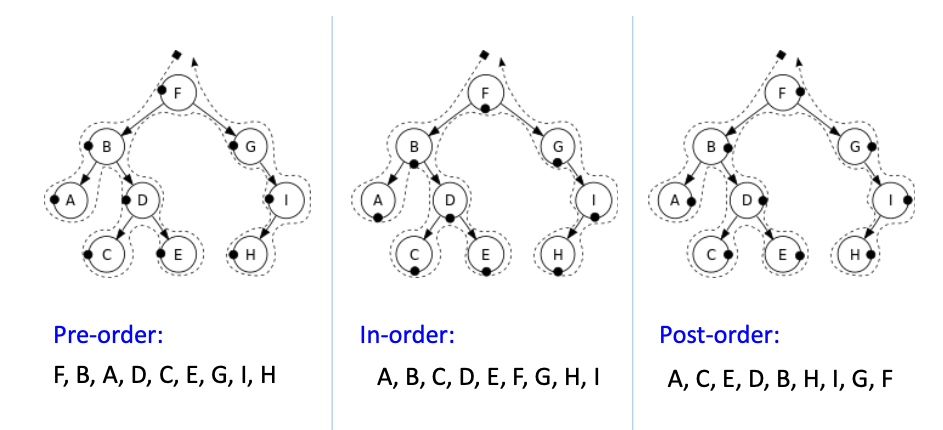
\includegraphics[width=12cm]{images/dfs_1.png}
        \end{center}
    \item (Spanning Tree): A spanning tree for a graph $G$ is a subgraph of $G$ that contains every vertex of $G$ and is a tree.
    \item Proposition 10.7.1:
        \\ \hspace*{3mm} (1) Every connected graph has a spanning tree.
        \\ \hspace*{3mm} (2) Any two spanning trees for a graph have the same number of edges.
    \item (Minimum Spanning Tree): A minimum spanning tree for a connected weighted graph is a spanning tree that has the least possible total weight compared to all other spanning trees for the graph.
    \item (Algorithms to get Minimum Spanning Tree):
        \begin{center}
            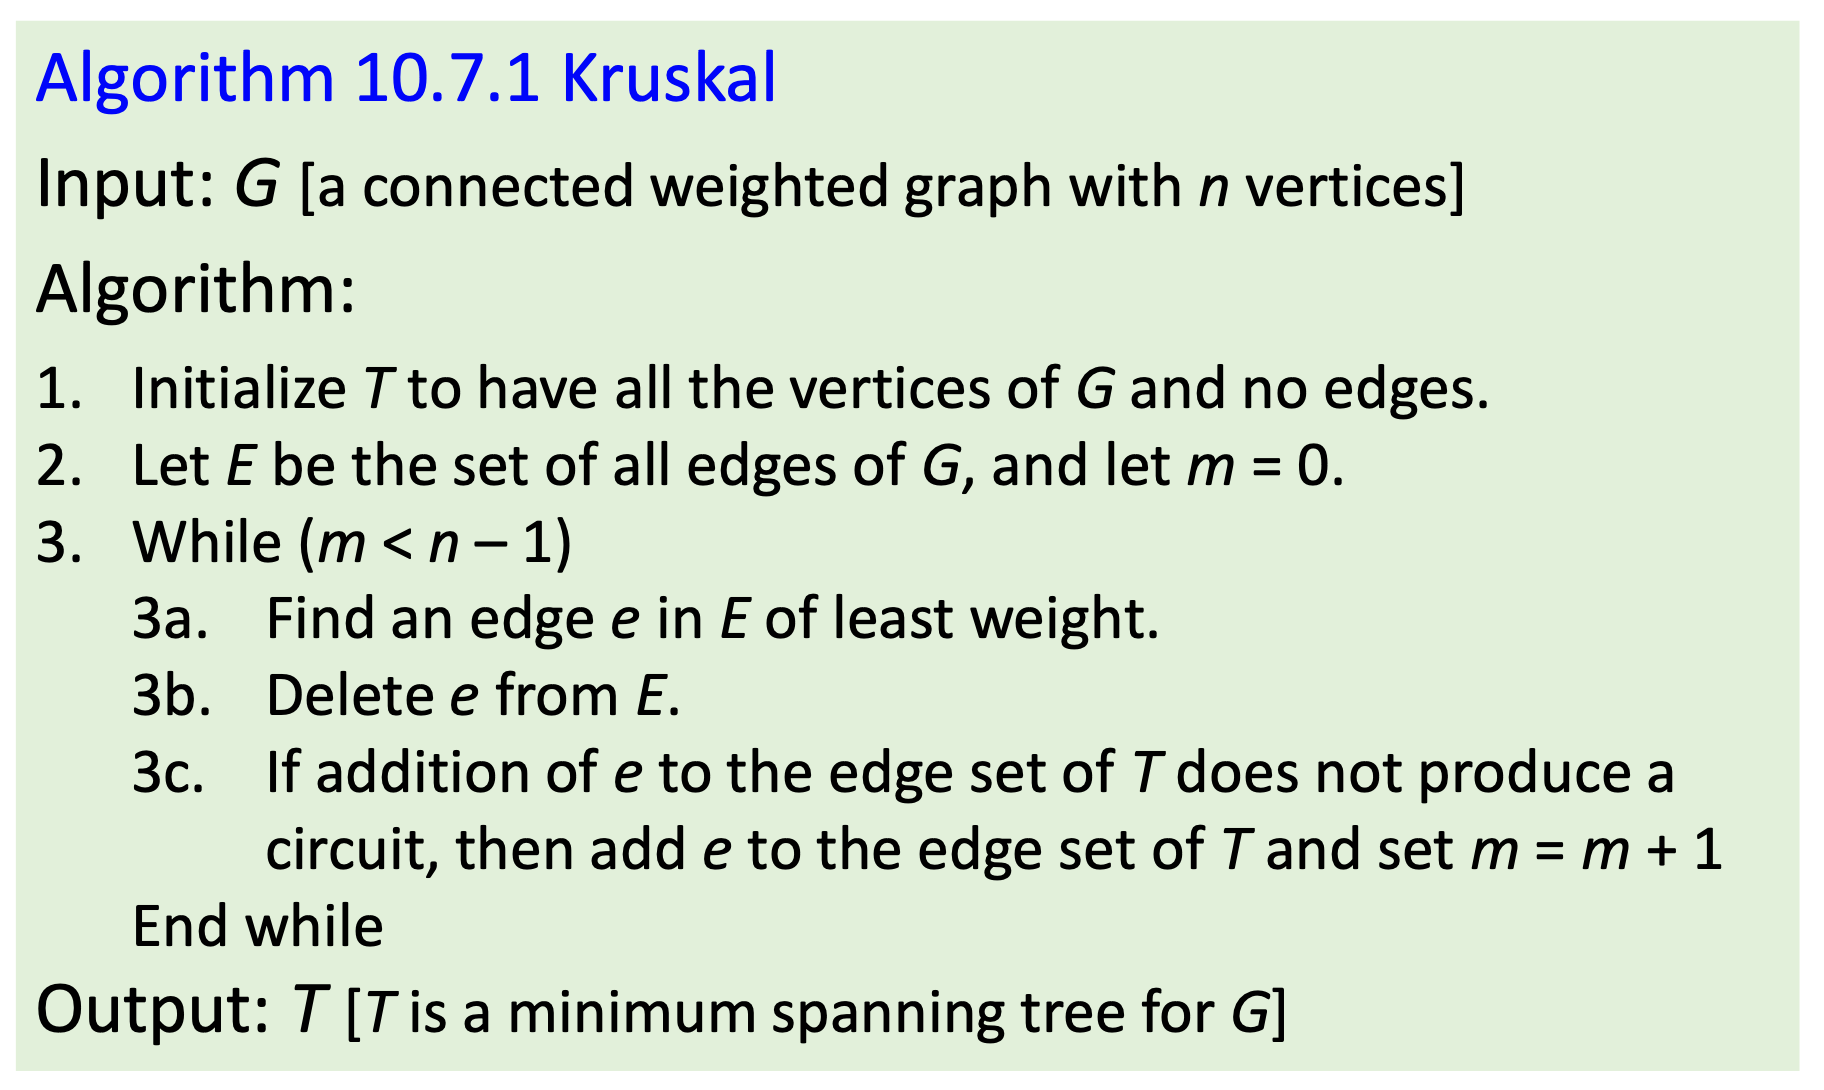
\includegraphics[width=8.5cm]{images/kruskal_algorithm.png}
            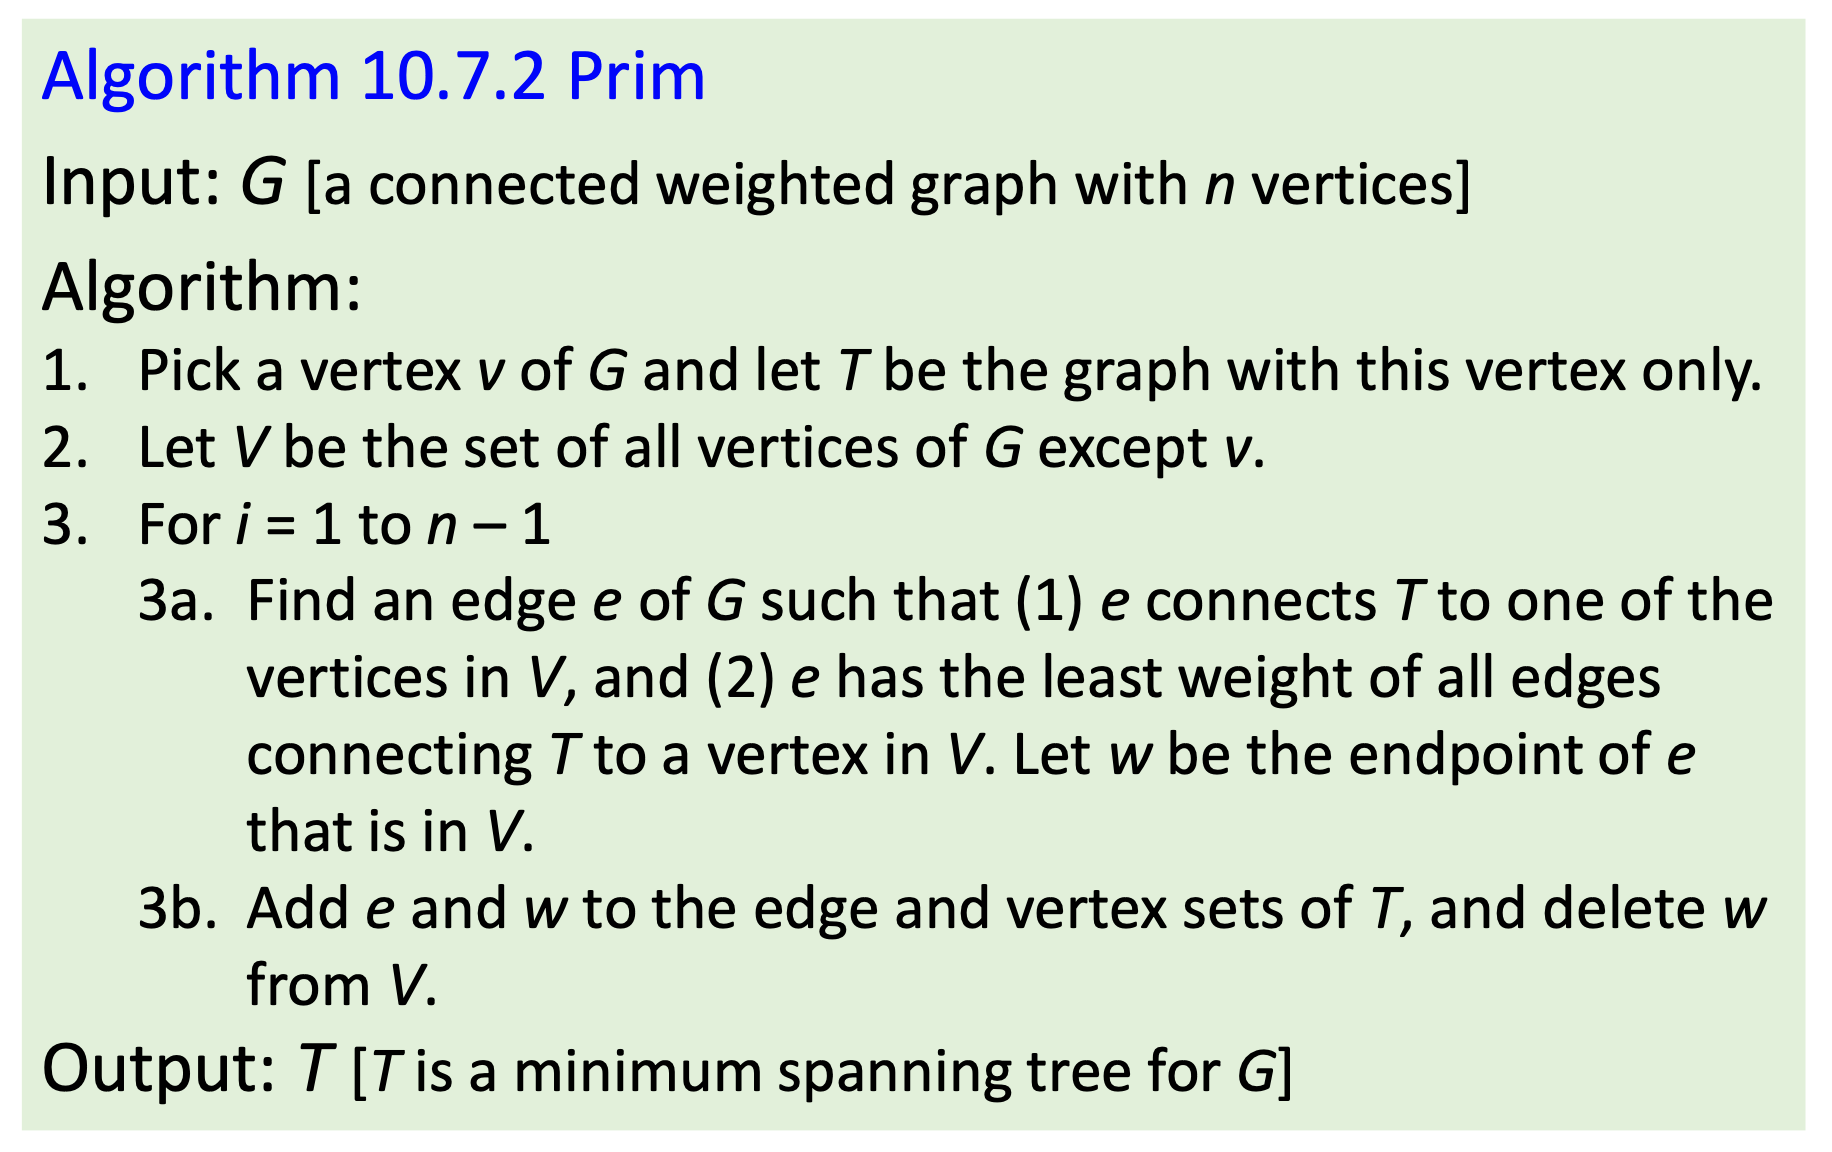
\includegraphics[width=8.5cm]{images/prim_algorithm.png}
        \end{center}
\end{itemize}

\end{document}